% !Mode:: "Tex:UTF-8"
\documentclass[10pt,a4paper]{article}\usepackage[]{graphicx}\usepackage[]{color}
%% maxwidth is the original width if it is less than linewidth
%% otherwise use linewidth (to make sure the graphics do not exceed the margin)
\makeatletter
\def\maxwidth{ %
  \ifdim\Gin@nat@width>\linewidth
    \linewidth
  \else
    \Gin@nat@width
  \fi
}
\makeatother

\definecolor{fgcolor}{rgb}{0.345, 0.345, 0.345}
\newcommand{\hlnum}[1]{\textcolor[rgb]{0.686,0.059,0.569}{#1}}%
\newcommand{\hlstr}[1]{\textcolor[rgb]{0.192,0.494,0.8}{#1}}%
\newcommand{\hlcom}[1]{\textcolor[rgb]{0.678,0.584,0.686}{\textit{#1}}}%
\newcommand{\hlopt}[1]{\textcolor[rgb]{0,0,0}{#1}}%
\newcommand{\hlstd}[1]{\textcolor[rgb]{0.345,0.345,0.345}{#1}}%
\newcommand{\hlkwa}[1]{\textcolor[rgb]{0.161,0.373,0.58}{\textbf{#1}}}%
\newcommand{\hlkwb}[1]{\textcolor[rgb]{0.69,0.353,0.396}{#1}}%
\newcommand{\hlkwc}[1]{\textcolor[rgb]{0.333,0.667,0.333}{#1}}%
\newcommand{\hlkwd}[1]{\textcolor[rgb]{0.737,0.353,0.396}{\textbf{#1}}}%
\let\hlipl\hlkwb

\usepackage{framed}
\makeatletter
\newenvironment{kframe}{%
 \def\at@end@of@kframe{}%
 \ifinner\ifhmode%
  \def\at@end@of@kframe{\end{minipage}}%
  \begin{minipage}{\columnwidth}%
 \fi\fi%
 \def\FrameCommand##1{\hskip\@totalleftmargin \hskip-\fboxsep
 \colorbox{shadecolor}{##1}\hskip-\fboxsep
     % There is no \\@totalrightmargin, so:
     \hskip-\linewidth \hskip-\@totalleftmargin \hskip\columnwidth}%
 \MakeFramed {\advance\hsize-\width
   \@totalleftmargin\z@ \linewidth\hsize
   \@setminipage}}%
 {\par\unskip\endMakeFramed%
 \at@end@of@kframe}
\makeatother

\definecolor{shadecolor}{rgb}{.97, .97, .97}
\definecolor{messagecolor}{rgb}{0, 0, 0}
\definecolor{warningcolor}{rgb}{1, 0, 1}
\definecolor{errorcolor}{rgb}{1, 0, 0}
\newenvironment{knitrout}{}{} % an empty environment to be redefined in TeX

\usepackage{alltt}
\usepackage{etoolbox}
\newtoggle{color}
%\togglefalse{color}
\toggletrue{color}
\usepackage{makeidx}
\newcommand{\idioma}{spanish}
\newcommand{\opcionesIdioma}{,es-nodecimaldot}
% !Mode:: "Tex:UTF-8"
%%%%%%%%%%%%%%%%%%%%%Carga de Packages
%%poner \newcommand{\idioma}{spanish} o \newcommand{\idioma}{english} en el documento
\usepackage{pdfsync}
\usepackage{srcltx}
\usepackage[\idioma\opcionesIdioma]{babel}
\usepackage[utf8x]{inputenc}
\usepackage[T1]{fontenc}
\usepackage{graphicx}
\graphicspath{{/users/fernando/figuras/}{./}{./figuras/}{/fernando/figuras/}{/fernando/figuras/jpg/}}
\usepackage{multicol}
\usepackage{epsfig}
%\usepackage{oberdiek}
\usepackage{listingsutf8}
\lstset{inputencoding=utf8/latin1}
%\lstset{extendedchars=true}
\lstset{ %
  language=R,                     % the language of the code
  basicstyle=\ttfamily\small,       % the size of the fonts that are used for the code
  numbers=left,                   % where to put the line-numbers
  numberstyle=\tiny\color{gray},  % the style that is used for the line-numbers
  stepnumber=1,                   % the step between two line-numbers. If it's 1, each line
                                  % will be numbered
  numbersep=5pt,                  % how far the line-numbers are from the code
  backgroundcolor=\color{white},  % choose the background color. You must add \usepackage{color}
  showspaces=false,               % show spaces adding particular underscores
  showstringspaces=false,         % underline spaces within strings
  showtabs=false,                 % show tabs within strings adding particular underscores
  frame=single,                   % adds a frame around the code
  rulecolor=\color{black},        % if not set, the frame-color may be changed on line-breaks within not-black text (e.g. commens (green here))
  tabsize=2,                      % sets default tabsize to 2 spaces
  %captionpos=,                   % sets the caption-position to bottom
  breaklines=true,                % sets automatic line breaking
  breakatwhitespace=false,        % sets if automatic breaks should only happen at whitespace
  %title=\lstname,                 % show the filename of files included with \lstinputlisting;
                                  % also try caption instead of title
  keywordstyle=\color{black},      % keyword style
  commentstyle=\color{Brown},   % comment style
  stringstyle=\color{black},      % string literal style
  escapeinside={\%*}{*)},         % if you want to add a comment within your code
  morekeywords={*,...},            % if you want to add more keywords to the set
  lineskip={-2.5pt} % single line spacing
}
%\usepackage{algorithm}
\usepackage{amsmath}
\usepackage{amsfonts}
\usepackage{amssymb}
\usepackage{amsthm}
\usepackage{fancybox}
\usepackage{fancyvrb}
\usepackage{rotating}
\usepackage{keystroke}
\usepackage{array}
\input{xy}
\xyoption{all}
%\usepackage[dvipsnames,usenames]{color}
\usepackage[usenames,dvipsnames,svgnames,table]{xcolor}
\usepackage{colortbl}
\usepackage{comment}
\excludecomment{spanish}
\excludecomment{english}
\includecomment{\idioma}

%\usepackage{noweb}
%\usepackage{clrscode}
\usepackage{eurosym}
\usepackage{wasysym}
\usepackage{multirow}
%\usepackage{margins}
\usepackage{lscape}
\usepackage{longtable}
\usepackage[normalem]{ulem}
\usepackage{xr-hyper}

%%NUEVO
\newcolumntype{C}{{\centering\arraybackslash}m{20mm}}
\newcommand{\centercell}[1]{\multicolumn{1}{c}{#1}}
\newcommand{\colHead}[1]{\centercell{\bfseries#1}}

\excludecomment{ocultar}


% Matriz (par‚ntesis)
\def\matr#1#2{\left(\begin{array}{#1}#2\end{array}\right)}
% Determinante (barras)
\def\deter#1#2{\left|\begin{array}{#1}#2\end{array}\right|}
% Sistema de ecuaciones. (llave a la izda.)
\def\seq#1#2{\left\{\begin{array}{#1}#2\end{array}\right.}
% Ecuaci\'on de varias lineas (sin llave a la izda.)
\def\evl#1#2{\begin{array}{#1}#2\end{array}}

%%%%%%%%%%%%%%%%%%%%%%%%%%%%%%%%%%%%%%%%%%%%%%
%%%%%%%%%%%%%%%%%%%%%%%%%%%%%%%%%%%%%%%%%%%%%%
%%%%%%%%%%%%%%%%% M\'{a}rgenes %%%%%%%%%%%%%%%%
%
%
%\parindent=0mm
%
%\textwidth=160mm
%\textheight=220mm
%\hoffset=-20mm
%\voffset=-15mm
%\parskip=0mm
\marginparsep=3mm
\marginparwidth=25mm
%
%%%%%%%%%%%%%%%%%%%%%%%%%%%% Contadores para listas de problemas
%\newcommand{\adc}{\addtocounter{enumi}{1}}
\newcommand{\adc}{\stepcounter{enumi}}
\newcommand{\adci}{\stepcounter{enumii}}
\newcommand{\xadc}{\addtocounter{xcounter}{1}}
\newcommand{\be}{\begin{enumerate}}
\newcommand{\ee}{\end{enumerate}}
\newcommand{\bi}{\begin{itemize}}
\newcommand{\ei}{\end{itemize}}
\newcounter{xcounter}


\newcommand{\nin}{{\noindent}}

%\newcounter{prob}{}
%\def\pr{\addtocounter{prob}{1}(\theprob)\ }
%\def\pr2{\addtocounter{prob}{2}(\theprob)\ }

%%%%%%%%%%%%%%%%%%%%%%%%%%%Fin de demostraciones, ejemplos, etc.
\newcommand{\fin}{$\square$}
%%%%%%%%%%%%%%%%%%%%%%%%%%Notaci\'{o}n matem\'{a}ticas generales
%\newcommand{\suc}[1]{\{#1_n\}}
%\newcommand{\sucn}[1]{\{#1_n\}_{n\in\mathbb{N}}}
%\newcommand{\ser}[1]{\sum #1_n}
%\newcommand{\sern}[1]{\sum_{n\geq 1} #1_n}
%\newcommand{\limn}{\lim_{n\rightarrow\infty}}
%\newcommand{\limnd}{\displaystyle\lim_{n\rightarrow\infty}}
%\newcommand{\mf}[1]{\mathbf{#1}}
%\newcommand{\mb}[1]{\mathbb{#1}}
%\newcommand{\D}[1]{\Dv_{\mf{#1}}}
%\newcommand{\bsigma}{\pmb{\sigma}}
%\newcommand{\bPhi}{\pmb{\Phi}}
%\newcommand{\vol}{\operatorname{vol}}
%\newcommand{\ldbr}{[\hspace{-1.5pt}[}
%\newcommand{\rdbr}{]\hspace{-1.5pt}]}
%\newcommand{\fpws}[2]{{#1}\ldbr{#2}\rdbr}
%\newcommand{\leftPui}{<\hspace{-3pt}<}
%\newcommand{\rightPui}{\hspace{-3pt}}
%\newcommand{\Pui}[2]{{#1}\hspace{-6pt}\leftPui{#2}\rightPui}
%\newcommand{\pdd}[2]{\dfrac{\partial{#1}}{\partial{#2}}}
%%%%%%%%%%Conjuntos de n\'{u}meros
\newcommand{\N}{\mathbb{N}} %conjunto de n\'{u}meros naturales
\newcommand{\Z}{\mathbb{Z}} %conjunto de n\'{u}meros enteros
\newcommand{\R}{\mathbb{R}} %conjunto de n\'{u}meros reales
\newcommand{\C}{\mathbb{C}} %conjunto de n\'{u}meros complejos
\newcommand{\Q}{\mathbb{Q}} %conjunto de n\'{u}meros racionales
\newcommand{\EP}{\mathbb{P}} %espacios proyectivos
\newcommand{\K}{\mathbb{K}} %cuerpo gen\'{e}rico
\newcommand{\A}{\mathbb{A}} %espacios afines

%%%%%%%%%%Estadistica
\newcommand{\MEAN}{\mathrm{E}}
\newcommand{\Var}{\mathrm{Var}}
\newcommand{\Cov}{\mathrm{Cov}}


%%%%%%%%%%Funciones
\def\arcsen{\operatorname{arcsen}}
\def\arctg{\operatorname{arctg}}
\def\argCosh{\operatorname{argCosh}}
\def\argSenh{\operatorname{argSenh}}
\def\argTgh{\operatorname{argTgh}}
\def\cosec{\operatorname{cosec}}
\def\Cosh{\operatorname{Cosh}}
\def\cotg{\operatorname{cotg}}
\def\Dv{\operatorname{D}}
\def\discrim{\operatorname{discrim}}
\def\dive{\operatorname{div}}
\def\dom{\operatorname{dom}}
\def\Ext{\operatorname{Ext}}
\def\Fr{\operatorname{Fr}}
\def\dder#1#2{\dfrac{d #1}{d #2} } %derivada en estilo display
\def\gr{\operatorname{gr}}
\def\grad{\operatorname{grad}}
\def\Imag{\operatorname{Im}}
\def\mcm{\operatorname{mcm}}
\def\rang{\operatorname{rang}}
\def\rot{\operatorname{rot}}
\def\sen{\operatorname{sen}}
\def\Senh{\operatorname{Senh}}
\def\sgn{\operatorname{sgn}}
\def\sig{\operatorname{sig}}
\def\tg{\operatorname{tg}}
\def\Tgh{\operatorname{Tgh}}
\def\E{\operatorname{E}}
\def\VAR{\operatorname{VAR}}
\newcommand{\margWeb}[2]{\noindent{#2}\marginpar[\hspace{-18mm}\link{#1}{WEB}]{\hspace*{-18mm}\link{#1}{WEB}}}

%%%%%%%%%%%%%%%%%%%%%%\'{A}lgebra conmutativa.
\def\multideg{\operatorname{multideg}} %multidegree of a polynomial
\def\LT{\operatorname{lt}} %leading term of a polynomial
\def\LC{\operatorname{lc}} %leading coefficient of a polynomial
\def\LM{\operatorname{lm}} %leading monomial of a polynomial
\def\Mexp{\mathbb{Z}^n_{\geq 0}} %set of multiexponents of monomials
\def\set#1{\left\{{#1}\right\}}
\newcommand{\vlist}[2]{\mbox{${#1}_{1},\ldots,{#1}_{#2}$}}
\def\deg{\operatorname{deg}} %grado de un polinomio
\def\cp{\operatorname{cp}} %coeficiente principal de un polinomio
\def\CP{\operatorname{cp}} %coeficiente principal de un polinomio
\def\set#1{\left\{{#1}\right\}} %llaves de conjunto
\newcommand{\V}{{\bf V}} %variedad de un conjunto de polinomios
\newcommand{\I}{{\bf I}} %ideal de un conjunto
\newcommand{\MCD}{\operatorname{mcd}} %m\'{a}ximo com\'{u}n divisor
\newcommand{\MCM}{\operatorname{mcm}} %m\'{\i}nimo com\'{u}n m\'{u}ltiplo
\newcommand{\LCM}{\operatorname{lcm}} %least common multiple
\newcommand{\GCD}{\operatorname{gcd}} %greatest common divisor
\newcommand{\Ker}{\operatorname{Ker}} %N\'{u}cleo
\newcommand{\IM}{\operatorname{IM}} %Imagen
\newcommand{\Rad}{\operatorname{Rad}} %radical de un ideal
\newcommand{\Jac}{\operatorname{Jac}} %radical de Jacobson de un anillo
\newcommand{\Ann}{\operatorname{Ann}} %anulador de un ideal
\newcommand{\Res}{\operatorname{Res}} %resultante de polinomios
\newcommand{\Mult}{\operatorname{mult}} %multiplicidad
\newcommand{\Gen}{\operatorname{Gen}} %g\'{e}nero
\newcommand{\Card}{\operatorname{Card}} %cardinal
\newcommand{\ord}{\operatorname{ord}} %orden
\newcommand{\prim}{\operatorname{prim}} %parte primitiva
\newcommand{\NP}{\operatorname{NP}} %NP idea
\newcommand{\cont}{\operatorname{cont}} %parte primitva
\newcommand{\pp}{\operatorname{pp}} %parte primitva
\newcommand{\PP}{\mathop{\mathrm{PP}}\nolimits}
\newcommand{\Int}{\operatorname{Int}}
\newcommand{\Ind}{\operatorname{index}}
\newcommand{\Lcoeff}{\operatorname{lc}} %leading coefficient of a polynomial
\newcommand{\Sqf}{\operatorname{Sqf}} %square free part of a polynomial

\def\pd#1#2{\frac{\partial #1}{\partial #2}} %derivada parcial
\def\mult{\text{mult}} %multiplicity
\def\Sing{\text{Sing}} %multiplicity
\def\Cl#1{\overline{#1}} %cierre topol\'{o}gico
\def\fobox#1{\begin{center}\fbox{$\displaystyle #1 $}\end{center}}

%\newcommand{\Ext}{\operatorname{Ext}}

%%%%%%%%%%%%%%%%%%%%%%%%
%% unpunto mayor que cdot, pero menor que bullet
\newcommand{\sbt}{\,\begin{picture}(-1,1)(-1,-3)\circle*{3}\end{picture}\ }

%%%%%%%%%%%%%%%%%%%%%%%%S\'{\i}mbolos rodeados de un c\'{\i}rculo
\def\circled#1{\xymatrix{*+[o][F]{#1}}}

%%%%%%%%%%%%%%%%%%%Geometr\'{\i}a
\newcommand{\CH}{{\cal CH}} %%cierre convexo

%%%%%%%%%%%%%%%%%%%%Tipos de letra especiales
%%Caligr\'{a}ficas
\newcommand{\cA}{{\cal A}}
\newcommand{\cB}{{\cal B}}
\newcommand{\cC}{{\cal C}}
\newcommand{\cD}{{\cal D}}
\newcommand{\cE}{{\cal E}}
\newcommand{\cF}{{\cal F}}
\newcommand{\cG}{{\cal G}}
\newcommand{\cH}{{\cal H}}
\newcommand{\cI}{{\cal I}}
\newcommand{\cJ}{{\cal J}}
\newcommand{\cK}{{\cal K}}
\newcommand{\cL}{{\cal L}}
\newcommand{\cM}{{\cal M}}
\newcommand{\cN}{{\cal N}}
\newcommand{\cO}{{\cal O}}
\newcommand{\cP}{{\cal P}}
\newcommand{\cQ}{{\cal Q}}
\newcommand{\cR}{{\cal R}}
\newcommand{\cS}{{\cal S}}
\newcommand{\cT}{{\cal T}}
\newcommand{\cU}{{\cal U}}
\newcommand{\cV}{{\cal V}}
\newcommand{\cW}{{\cal W}}
\newcommand{\cX}{{\cal X}}
\newcommand{\cY}{{\cal Y}}
\newcommand{\cZ}{{\cal Z}}

%%%%%%%%%%%%%%%%%%%%%%%%%%Notaci\'{o}n matem\'{a}ticas generales
\newcommand{\sucn}[1]{\{#1_n\}_{n\in\mathbb{N}}}
\newcommand{\ser}[1]{\sum #1_n}
\newcommand{\sern}[1]{\sum_{n\geq 1} #1_n}
\newcommand{\limn}{\lim_{n\rightarrow\infty}}
\newcommand{\mf}[1]{\mathbf{#1}}
\newcommand{\mb}[1]{\mathbb{#1}}
\newcommand{\D}[1]{\Dv_{\mf{#1}}}
\newcommand{\bsigma}{\pmb{\sigma}}
\newcommand{\bPhi}{\pmb{\Phi}}
\newcommand{\vol}{\operatorname{vol}}
\newcommand{\ldbr}{[\hspace{-1.5pt}[}
\newcommand{\rdbr}{]\hspace{-1.5pt}]}
\newcommand{\fpws}[2]{{#1}\ldbr{#2}\rdbr}
\newcommand{\leftPui}{<\hspace{-3pt}<}
\newcommand{\rightPui}{\hspace{-3pt}}
\newcommand{\Pui}[2]{{#1}\hspace{-6pt}\leftPui{#2}\rightPui}
\newcommand{\pdd}[2]{\dfrac{\partial{#1}}{\partial{#2}}}


%\newcounter{contEnlace}

%\newcommand{\pendiente}{\textcolor{purple}{PENDIENTE: }}
%\newcommand{\link}[2]{\textcolor{blue}{{\href{#1}{#2}}}}


\iftoggle{color}{%
  % color version
  \newcommand{\pendiente}{\textcolor{red}{PENDIENTE: }}
  \newcommand{\link}[2]{\textcolor{blue}{{\href{#1}{#2}}}}
  \newcommand{\fichero}[2]{\textattachfile{#1}{\textcolor{blue}{#2}}}
  \newcommand{\otrofichero}[2]{\textattachfile{./datos/#1}{\textcolor{blue}{#2}}}
}{%
  % b/w version
  \newcommand{\pendiente}{\textcolor{black}{\underline{PENDIENTE:} }}
  \newcommand{\link}[2]{\textcolor{black}{{\href{#1}{\underline{#2}}}}}
  \newcommand{\fichero}[2]{\textattachfile{#1}{\textcolor{black}{\underline{#2}}}}
  \newcommand{\otrofichero}[2]{\textattachfile{./datos/#1}{\textcolor{black}{\underline{#2}}}}
}



%{\textcolor{blue}{{\href{#1}{#2}}}}

%%%%%%%%%%%%%%%%%%COLORES

\DefineNamedColor{named}{Brown}{cmyk}{0,0.81,1,0.60}
\definecolor{Gris050}{gray}{0.50}
\definecolor{Gris025}{gray}{0.75}
\definecolor{Gris010}{gray}{0.90}


%%%%%%%%%%%%%%%%%%%%%Package Algorithms
%\begin{spanish}
%\renewcommand{\algorithmicrequire}{{precondici\'{o}n:}}
%\renewcommand{\algorithmicensure}{{postcondici\'{o}n:}}
%\renewcommand{\algorithmicend}{{fin}}
%\renewcommand{\algorithmicif}{{si}}
% \renewcommand{\algorithmicthen}{{entonces}}
% \renewcommand{\algorithmicelse}{{si no}}
% \renewcommand{\algorithmicelsif}{\algorithmicelse\ \algorithmicif}
% \renewcommand{\algorithmicendif}{\algorithmicend\ \algorithmicif}
% \renewcommand{\algorithmicfor}{{para}}
% \renewcommand{\algorithmicforall}{{para todo}}
% \renewcommand{\algorithmicdo}{{hacer}}
% \renewcommand{\algorithmicendfor}{\algorithmicend\ \algorithmicfor}
% \renewcommand{\algorithmicwhile}{{mientras}}
% \renewcommand{\algorithmicendwhile}{\algorithmicend\ \algorithmicwhile}
% \renewcommand{\algorithmicrepeat}{{repetir}}
% \renewcommand{\algorithmicuntil}{{hasta}}
% \end{spanish}

%%%%%%%%%%%%%%%%%%%%%%%%%%%%%%%%%%Package Amsthm
\begin{spanish}
%\theoremstyle{definition}% default
\theoremstyle{plain}
\newtheorem{thm}{Teorema}[section]
\newtheorem{teo}{Teorema}[section]
\newtheorem{teorema}{Teorema}[section]
\newtheorem{lem}[thm]{Lema}
\newtheorem{lema}[thm]{Lema}
\newtheorem{prop}[thm]{Proposici\'{o}n}
\newtheorem{proposicion}[thm]{Proposici\'{o}n}
\newtheorem{cor}[thm]{Corolario}
\newtheorem{corolario}[thm]{Corolario}
\newtheorem*{KL}{Klein's Lemma}
%\theoremstyle{definition}
\newtheorem{defn}[thm]{Definici\'{o}n}
\newtheorem{definicion}[thm]{Definici\'{o}n}
\newtheorem{conj}[thm]{Conjetura}
\newtheorem{conjetura}[thm]{Conjetura}
\newtheorem{definicionInformal}[thm]{Definición Informal}
\newtheorem{exmp}[thm]{Ejemplo}
\newtheorem{ejemplo}[thm]{Ejemplo}
\newtheorem{Ejemplo}[thm]{Ejemplo}
\newtheorem{ejem}[thm]{Ejemplo}
\newtheorem{ejercicio}{Ejercicio}
%\theoremstyle{remark}
\newtheorem*{rem}{Observaci\'{o}n}
\newtheorem{observacion}[thm]{Observaci\'{o}n}
\newtheorem*{note}{Nota}
\newtheorem{nota}[thm]{Nota}
\newtheorem{case}[thm]{Caso}
\newtheorem{caso}[thm]{Caso}
\newtheorem{regla}[thm]{Regla}

\theoremstyle{remark}
\newtheorem{enlace}{$\bullet$ }
\end{spanish}

\begin{english}
\theoremstyle{plain}% default
%\theoremstyle{definition}
\newtheorem{thm}{Theorem}[section]
\newtheorem{lem}[thm]{Lemma}
\newtheorem{prop}[thm]{Proposition}
\newtheorem{cor}[thm]{Corollary}
\newtheorem*{KL}{Klein's Lemma}
\newtheorem{defn}[thm]{Definition}
\newtheorem{conj}[thm]{Conjecture}
\newtheorem{exmp}[thm]{Example}
\theoremstyle{remark}
\newtheorem*{rem}{Remark}
\newtheorem*{note}{Note}
\newtheorem{case}{Case}
\end{english}

%%%%%%%%%%%%%%%Package Listings
%\lstset{showstringspaces=false}
%\newcommand{\PAS}[1]{\lstinline@#1@}
%\newcommand{\CPP}[1]{\lstinline@#1@}


%%%%%%%%%%%%Estilo para bibliograf\'{\i}a

%\bibliographystyle{plain}

%%%%%%%%%%%%Mis anotaciones
\newcommand{\Pendiente}[1]{\textcolor{red}{Pendiente: #1}}
%\newcommand{\Pendiente}{\textcolor{purple}{Pendiente: }}

\newcommand{\fernando}[1]{\textcolor{red}{Fernando: #1}}

%%%%%%%%%%%%%%%% Enlace al indice
%\renewcommand{\chaptermark}[1]{\markboth{\chaptername\ \thechapter.#1 \ref{index}}{}}

%%%%%%%%%%%%%%%%%%Traducci\'{o}n de clrscode
%\renewcommand{\For}{\textbf{Para} }
%\renewcommand{\To}{\textbf{hasta} }
%\renewcommand{\By}{\textbf{incremento} }
%\renewcommand{\Downto}{\textbf{downto} }
%\renewcommand{\While}{\textbf{mientras} }
%\renewcommand{\Repeat}{\textbf{repetir}\\\addtocounter{indent}{1}}
%\renewcommand{\Until}{\kill\addtocounter{indent}{-1}\liprint\\\textbf{hasta que}\hspace*{-0.7em}\'}
%\renewcommand{\If}{\textbf{si} }
%\renewcommand{\Then}{\\textbf{entonces}\hspace{13mm}\\addtocounter{indent}{1}}
%\renewcommand{\Else}{\kill\addtocounter{indent}{-1}\liprint\\textbf{sino}\\addtocounter{indent}{1}}
%\renewcommand{\End}{\addtocounter{indent}{-1}}
%\renewcommand{\ElseIf}{\kill\addtocounter{indent}{-1}\liprint\textbf{sino si} }
%\renewcommand{\ElseNoIf}{\kill\addtocounter{indent}{-1}\liprint\textbf{si no}\addtocounter{indent}{1}}
%\renewcommand{\Do}{\\\textbf{hacer}\hspace*{-0.7em}\'\addtocounter{indent}{1}}
%\renewcommand{\Return}{\textbf{devolver} }
%\renewcommand{\Comment}{$\hspace*{-0.075em}\rhd$ }
%\renewcommand{\RComment}{\`\Comment}
%\renewcommand{\Goto}{\textbf{Ir a} }
%\renewcommand{\Error}{\textbf{error} }


%%%%%%%%%%%%%%%%%%%%%%%%%%%%%%%%%%%%%%%%%%%%%%%%%%%%%%%%%%%%%%%
%Cabecera para ejercicios
%\documentclass[11pt]{article}
%\newcommand{\idioma}{spanish}
%\input definiciones
%
%\textwidth=160mm \textheight=240mm \hoffset=-20mm \voffset=-30mm
%%\parskip=0mm
%%\marginparsep=-25mm \evensidemargin=82pt\evensidemargin=44pt
%
%
%\includecomment{solucion}
%%\excludecomment{solucion}

%%Compatibilidad con documentos antiguos
\newcounter{prob}{}
\def\pr{\noindent\addtocounter{prob}{1}(\theprob)\ }
\def\bepro{ \setcounter{prob}{0}}

%%Compatibilidad con documentos antiguos
% \def\ojo#1{
% \noindent$\btr$#1
% \marginpar[
% {GeoGebra}]
% {GeoGebra}}

% \def\atencion#1{\noindent #1
% \marginpar[
% {\includegraphics*[scale=1,width=1.2cm,keepaspectratio=true]{./datos/hipoizda}}]
% {\includegraphics*[scale=1,width=1.2cm,keepaspectratio=true]{./datos/hipodcha}}}


\def\Rlogo#1{\noindent #1
\marginpar[
{\includegraphics*[scale=1,width=1.5cm,keepaspectratio=true]{./datos/Rlogo.jpg}}]
{\includegraphics*[scale=1,width=1.5cm,keepaspectratio=true]{./datos/Rlogo.jpg}}}

\def\calcLogo#1{#1}

%\def\calcLogo#1{\noindent #1
%\marginpar[
%{\includegraphics*[scale=1,width=1.2cm,keepaspectratio=true]{./datos/LogoHojaCalculo.png}}]
%{\includegraphics*[scale=1,width=1.2cm,keepaspectratio=true]{./datos/LogoHojaCalculo.png}}}


\def\ninja#1{\noindent #1
\marginpar[ {\includegraphics*[scale=1,width=1.2cm,keepaspectratio=true]{../fig/ninja_desk.png}}]
{\includegraphics*[scale=1,width=1.2cm,keepaspectratio=true]{../fig/ninja_desk.png}}}

\def\buda#1{\noindent #1
\marginpar[ {\includegraphics*[scale=1,width=1.2cm,keepaspectratio=true]{../fig/Computer-Buddha.png}}]
{\includegraphics*[scale=1,width=1.2cm,keepaspectratio=true]{../fig/Computer-Buddha.png}}}


\def\puffin#1{\noindent #1
\marginpar[ {\includegraphics*[scale=1,width=1.2cm,keepaspectratio=true]{../fig/frailecillo3.png}}]
{\includegraphics*[scale=1,width=1.2cm,keepaspectratio=true]{../fig/frailecillo3-dcha.png}}}


\def\atencion{
\marginpar[
{\includegraphics*[scale=1,width=2cm,keepaspectratio=true]{./datos/hipoizda}}]
{\includegraphics*[scale=1,width=2cm,keepaspectratio=true]{./datos/hipodcha}}}


\def\ojo#1{
\noindent #1
\marginpar[
{\includegraphics*[scale=1,width=1.5cm,keepaspectratio=true]{./datos/hipoojoi}}]
{\includegraphics*[scale=1,width=1.5cm,keepaspectratio=true]{./datos/hipoojod}}}

\def\ojo2{
\marginpar[
{\includegraphics*[scale=1,width=1.5cm,keepaspectratio=true]{./datos/hipoojoi}}]
{\includegraphics*[scale=1,width=1.5cm,keepaspectratio=true]{./datos/hipoojod}}}


\def\lio#1{
\noindent$\btr$#1
\marginpar{\includegraphics*[scale=1,width=1.1cm,keepaspectratio=true]{./datos/hipolio}}}

\def\cuentas{
\marginpar{\includegraphics*[scale=1,width=1.3cm,keepaspectratio=true]{./datos/hipocuen}}}

\def\pensar{
\marginpar{\includegraphics*[scale=1,width=1.5cm,keepaspectratio=true]{./datos/hipopens}}}

\def\facil{
\marginpar{\includegraphics*[scale=1,width=2cm,keepaspectratio=true]{./datos/hipofcil}}}



\newcommand{\WikipediaLogo}{\marginpar{\includegraphics*[scale=1,width=1.2cm,keepaspectratio=true]{./datos/LogoWikipedia}}}
\newcommand{\MoodleLogo}{\marginpar{\includegraphics*[scale=1,width=1.2cm,keepaspectratio=true]{./datos/MoodleLogo}}}
\newcommand{\WirisGeoGebraLogo}{\marginpar{\includegraphics*[scale=1,width=1.2cm,keepaspectratio=true]{./datos/WirisGeoGebraLogo}}}
\newcommand{\WirisLogo}{\marginpar{\includegraphics*[scale=1,width=1.2cm,keepaspectratio=true]{./datos/WirisLogo}}}
\newcommand{\GeoGebraLogo}{\marginpar{\includegraphics*[scale=1,width=1.2cm,keepaspectratio=true]{./datos/GeoGebra-Logo}}}


\newcommand{\enObras}[1]{\includegraphics*[scale=1,width=0.5cm,keepaspectratio=true]{./datos/obras.png}\textcolor{blue}{#1}}



\newcommand{\GeoGebra}[2]{\noindent #1
\marginpar[{\link{#2}{\small Moodle}\\\includegraphics*[scale=1,width=1.2cm,keepaspectratio=true]{./datos/MoodleLogo}}]{\link{#2}{\small Moodle}\\\includegraphics*[scale=1,width=1.2cm,keepaspectratio=true]{./datos/MoodleLogo}}}

\newcommand{\Moodle}[2]{\noindent #1
\marginpar[{\link{#2}{\small Moodle}\\\includegraphics*[scale=1,width=1.2cm,keepaspectratio=true]{./datos/MoodleLogo}}]{\link{#2}{\small Moodle}\\\includegraphics*[scale=1,width=1.2cm,keepaspectratio=true]{./datos/MoodleLogo}}}

\newcommand{\Wikipedia}[2]{\noindent #1
\marginpar[{\link{#2}{\small Wikipedia}\\\includegraphics*[scale=1,width=1.2cm,keepaspectratio=true]{./datos/LogoWikipedia}}]{\link{#2}{\small Wikipedia}\\\includegraphics*[scale=1,width=1.2cm,keepaspectratio=true]{./datos/LogoWikipedia}}}


\newcommand{\pder}[2]{\frac{\partial #1}{\partial #2}}

%%%%%%%%%%%%%%%%%%%%%%%%%%%%%%%%%%%%%%%%%%%%%%
%%%%%%%%%%%%%%%%%%%%%%%%%%%%%%%%%%%%%%%%%%%%%%%
%%%%%%%%%%%%%%%%%% M\'{a}rgenes %%%%%%%%%%%%%%%%
%%
%%
%%\parindent=0mm
%%
%\textwidth=160mm \textheight=220mm \hoffset=-20mm \voffset=-15mm
%\parskip=0mm
%\marginparsep=-25mm
%%
%%%%%%%%%%%%%%%%%%%%%%%%%%%%% Contadores para listas de problemas
%%\newcommand{\adc}{\addtocounter{enumi}{1}}
%\newcommand{\adc}{\stepcounter{enumi}}
%\newcommand{\adci}{\stepcounter{enumii}}
%\newcommand{\xadc}{\addtocounter{xcounter}{1}}
%\newcommand{\be}{\begin{enumerate}}
%\newcommand{\ee}{\end{enumerate}}
%\newcommand{\bi}{\begin{itemize}}
%\newcommand{\ei}{\end{itemize}}
%\newcounter{xcounter}
%\newcounter{probl}
%\setcounter{probl}{0}
%\newcommand{\pro}{\addtocounter{probl}{1}}
%\newcommand{\pr}{{\pro}{(\theprobl.)}}
%%%%%%%%%%%%%%%%%%%%%%%%%%%%Fin de demostraciones, ejemplos, etc.
%\newcommand{\fin}{$\square$}
%%%%%%%%%%%%%%%%%%%%%%%%%%%Notaci\'{o}n matem\'{a}ticas generales
%\newcommand{\suc}[1]{\{#1_n\}}
%\newcommand{\sucn}[1]{\{#1_n\}_{n\in\mathbb{N}}}
%\newcommand{\ser}[1]{\sum #1_n}
%\newcommand{\sern}[1]{\sum_{n\geq 1} #1_n}
%\newcommand{\limn}{\lim_{n\rightarrow\infty}}
%\newcommand{\mf}[1]{\mathbf{#1}}
%\newcommand{\mb}[1]{\mathbb{#1}}
%\newcommand{\D}[1]{\Dv_{\mf{#1}}}
%\newcommand{\bsigma}{\pmb{\sigma}}
%\newcommand{\bPhi}{\pmb{\Phi}}
%\newcommand{\vol}{\operatorname{vol}}
%\newcommand{\ldbr}{[\hspace{-1.5pt}[}
%\newcommand{\rdbr}{]\hspace{-1.5pt}]}
%\newcommand{\fpws}[2]{{#1}\ldbr{#2}\rdbr}
%\newcommand{\leftPui}{<\hspace{-3pt}<}
%\newcommand{\rightPui}{\hspace{-3pt}}
%\newcommand{\Pui}[2]{{#1}\hspace{-6pt}\leftPui{#2}\rightPui}
%\newcommand{\pdd}[2]{\dfrac{\partial{#1}}{\partial{#2}}}
%%%%%%%%%%%Conjuntos de n\'{u}meros
%\newcommand{\N}{\mathbb{N}} %conjunto de n\'{u}meros naturales
%\newcommand{\Z}{\mathbb{Z}} %conjunto de n\'{u}meros enteros
%\newcommand{\R}{\mathbb{R}} %conjunto de n\'{u}meros reales
%\newcommand{\C}{\mathbb{C}} %conjunto de n\'{u}meros complejos
%\newcommand{\Q}{\mathbb{Q}} %conjunto de n\'{u}meros racionales
%\newcommand{\EP}{\mathbb{P}} %espacios proyectivos
%\newcommand{\K}{\mathbb{K}} %cuerpo gen\'{e}rico
%\newcommand{\A}{\mathbb{A}} %espacios afines
%%%%%%%%%%%Funciones
%\def\arcsen{\operatorname{arcsen}}
%\def\arctg{\operatorname{arctg}}
%\def\argCosh{\operatorname{argCosh}}
%\def\argSenh{\operatorname{argSenh}}
%\def\argTgh{\operatorname{argTgh}}
%\def\cosec{\operatorname{cosec}}
%\def\Cosh{\operatorname{Cosh}}
%\def\cotg{\operatorname{cotg}}
%\def\Dv{\operatorname{D}}
%\def\discrim{\operatorname{discrim}}
%\def\dive{\operatorname{div}}
%\def\dom{\operatorname{dom}}
%\def\Ext{\operatorname{Ext}}
%\def\Fr{\operatorname{Fr}}
%\def\gr{\operatorname{gr}}
%\def\grad{\operatorname{grad}}
%\def\Imag{\operatorname{Im}}
%\def\mcm{\operatorname{mcm}}
%\def\rang{\operatorname{rang}}
%\def\rot{\operatorname{rot}}
%\def\sen{\operatorname{sen}}
%\def\Senh{\operatorname{Senh}}
%\def\sgn{\operatorname{sgn}}
%\def\sig{\operatorname{sig}}
%\def\tg{\operatorname{tg}}
%\def\Tgh{\operatorname{Tgh}}
%\def\E{\operatorname{E}}
%\def\VAR{\operatorname{VAR}}
%
%%%%%%%%%%%%%%%%%%%%%%%\'{A}lgebra conmutativa.
%\def\multideg{\operatorname{multideg}} %multidegree of a polynomial
%\def\LT{\operatorname{lt}} %leading term of a polynomial
%\def\LC{\operatorname{lc}} %leading coefficient of a polynomial
%\def\LM{\operatorname{lm}} %leading monomial of a polynomial
%\def\Mexp{\mathbb{Z}^n_{\geq 0}} %set of multiexponents of monomials
%\def\set#1{\left\{{#1}\right\}}
%\newcommand{\vlist}[2]{\mbox{${#1}_{1},\ldots,{#1}_{#2}$}}
%\def\deg{\operatorname{deg}} %grado de un polinomio
%\def\cp{\operatorname{cp}} %coeficiente principal de un polinomio
%\def\CP{\operatorname{cp}} %coeficiente principal de un polinomio
%\def\set#1{\left\{{#1}\right\}} %llaves de conjunto
%\newcommand{\V}{{\bf V}} %variedad de un conjunto de polinomios
%\newcommand{\I}{{\bf I}} %ideal de un conjunto
%\newcommand{\MCD}{\operatorname{mcd}} %m\'{a}ximo com\'{u}n divisor
%\newcommand{\MCM}{\operatorname{mcm}} %m\'{\i}nimo com\'{u}n m\'{u}ltiplo
%\newcommand{\LCM}{\operatorname{lcm}} %least common multiple
%\newcommand{\GCD}{\operatorname{gcd}} %greatest common divisor
%\newcommand{\Ker}{\operatorname{Ker}} %N\'{u}cleo
%\newcommand{\IM}{\operatorname{IM}} %Imagen
%\newcommand{\Rad}{\operatorname{Rad}} %radical de un ideal
%\newcommand{\Jac}{\operatorname{Jac}} %radical de Jacobson de un anillo
%\newcommand{\Ann}{\operatorname{Ann}} %anulador de un ideal
%\newcommand{\Res}{\operatorname{Res}} %resultante de polinomios
%\newcommand{\Mult}{\operatorname{mult}} %multiplicidad
%\newcommand{\Gen}{\operatorname{Gen}} %g\'{e}nero
%\newcommand{\Card}{\operatorname{Card}} %cardinal
%\newcommand{\ord}{\operatorname{ord}} %orden
%\newcommand{\prim}{\operatorname{prim}} %parte primitiva
%\newcommand{\NP}{\operatorname{NP}} %NP idea
%\newcommand{\cont}{\operatorname{cont}} %parte primitva
%\newcommand{\pp}{\operatorname{pp}} %parte primitva
%\newcommand{\PP}{\mathop{\mathrm{PP}}\nolimits}
%\newcommand{\Int}{\operatorname{Int}}
%\newcommand{\Ind}{\operatorname{index}}
%\newcommand{\Lcoeff}{\operatorname{lc}} %leading coefficient of a polynomial
%\newcommand{\Sqf}{\operatorname{Sqf}} %square free part of a polynomial
%
%\def\pd#1#2{\frac{\partial #1}{\partial #2}} %derivada parcial
%\def\mult{\text{mult}} %multiplicity
%\def\Sing{\text{Sing}} %multiplicity
%\def\Cl#1{\overline{#1}} %cierre topol\'{o}gico
%
%%\newcommand{\Ext}{\operatorname{Ext}}
%
%%%%%%%%%%%%%%%%%%%%%%%%%S\'{\i}mbolos rodeados de un c\'{\i}rculo
%\def\circled#1{\xymatrix{*+[o][F]{#1}}}
%
%%%%%%%%%%%%%%%%%%%%Geometr\'{\i}a
%\newcommand{\CH}{{\cal CH}} %%cierre convexo
%
%%%%%%%%%%%%%%%%%%%%%Tipos de letra especiales
%%%Caligr\'{a}ficas
%\newcommand{\cA}{{\cal A}}
%\newcommand{\cB}{{\cal B}}
%\newcommand{\cC}{{\cal C}}
%\newcommand{\cD}{{\cal D}}
%\newcommand{\cE}{{\cal E}}
%\newcommand{\cF}{{\cal F}}
%\newcommand{\cG}{{\cal G}}
%\newcommand{\cH}{{\cal H}}
%\newcommand{\cI}{{\cal I}}
%\newcommand{\cJ}{{\cal J}}
%\newcommand{\cK}{{\cal K}}
%\newcommand{\cL}{{\cal L}}
%\newcommand{\cM}{{\cal M}}
%\newcommand{\cN}{{\cal N}}
%\newcommand{\cO}{{\cal O}}
%\newcommand{\cP}{{\cal P}}
%\newcommand{\cQ}{{\cal Q}}
%\newcommand{\cR}{{\cal R}}
%\newcommand{\cS}{{\cal S}}
%\newcommand{\cT}{{\cal T}}
%\newcommand{\cU}{{\cal U}}
%\newcommand{\cV}{{\cal V}}
%\newcommand{\cW}{{\cal W}}
%\newcommand{\cX}{{\cal X}}
%\newcommand{\cY}{{\cal Y}}
%\newcommand{\cZ}{{\cal Z}}
%
%
%%%%%%%%%%%%%%%%%%%COLORES
%
%\DefineNamedColor{named}{Brown}{cmyk}{0,0.81,1,0.60}
%\definecolor{Gris050}{gray}{0.50}
%\definecolor{Gris025}{gray}{0.50}
%
%
%%\theoremstyle{plain}
%%\newtheorem{thm}{Teorema}[section]
%%%\newtheorem{teo}{Teorema}[section]
%%\newtheorem{lem}[thm]{Lema}
%%\newtheorem{prop}[thm]{Proposici\'{o}n}
%%\newtheorem{cor}[thm]{Corolario}
%%\newtheorem*{KL}{Klein's Lemma}
%%%\theoremstyle{definition}
%%\newtheorem{defn}[thm]{Definici\'{o}n}
%%\newtheorem{conj}[thm]{Conjetura}
%%\newtheorem{exmp}[thm]{Ejemplo}
%%\newtheorem{ejem}[thm]{Ejemplo}
%%\theoremstyle{remark}
%%\newtheorem*{rem}{Observaci\'{o}n}
%%\newtheorem*{note}{Nota}
%%\newtheorem{case}{Caso}
%%\newtheorem{regla}[thm]{Regla}
%
%\theoremstyle{plain}
%\newtheorem{thm}{Teorema}%[subsection]
%%\newtheorem{teo}{Teorema}[section]
%%\newtheorem{teorema}{Teorema}[section]
%\newtheorem{lem}[thm]{Lema}
%\newtheorem{lema}[thm]{Lema}
%\newtheorem{prop}[thm]{Proposici\'{o}n}
%\newtheorem{proposicion}[thm]{Proposici\'{o}n}
%\newtheorem{cor}[thm]{Corolario}
%\newtheorem{corolario}[thm]{Corolario}
%\newtheorem*{KL}{Klein's Lemma}
%%\theoremstyle{definition}
%\newtheorem{defn}[thm]{Definici\'{o}n}
%\newtheorem{definicion}[thm]{Definici\'{o}n}
%\newtheorem{conj}[thm]{Conjetura}
%\newtheorem{conjetura}[thm]{Conjetura}
%\newtheorem{exmp}[thm]{Ejemplo}
%\newtheorem{ejemplo}[thm]{Ejemplo}
%\newtheorem{ejem}[thm]{Ejemplo}
%\newtheorem{ejercicio}[thm]{Ejemplo}
%\theoremstyle{remark}
%\newtheorem*{rem}{Observaci\'{o}n}
%\newtheorem*{observacion}{Observaci\'{o}n}
%\newtheorem*{note}{Nota}
%\newtheorem*{nota}{Nota}
%\newtheorem{case}{Caso}
%\newtheorem{caso}{Caso}
%\newtheorem{regla}[thm]{Regla}
%
%%%%%%%%%%%%%Estilo para bibliograf\'{\i}a
%
%\bibliographystyle{plain}
%
%%%%%%%%%%%%%Mis anotaciones
%\newcommand{\Pendiente}{\textcolor{blue}{Pendiente: }}

\renewcommand{\listtablename}{Indice de tablas}
\renewcommand{\tablename}{Tabla}


%%%%%%%%%%%%%%%%%%%%%%%%%%%%%%%%%%%%%%%%%%%%%%%%%%%
\def\indexCond#1{
\ifnumcomp{\value{chapter}}{<}{3}{
        \index{#1}
    }
    {
        \index{#1}%% nothing is done
    }
}


\usepackage[pageanchor=true]{hyperref}
\makeindex

\usepackage{pdfpages}

%\input{sahp}
\includecomment{com}
%\excludecomment{com}
%\usepackage[dvips]{hyperref}
%\usepackage{pstricks}
\usepackage{attachfile}

\textwidth=150mm \textheight=260mm
\hoffset=-1cm
\voffset=-25mm
%\textwidth=160mm \textheight=240mm \hoffset=-20mm \voffset=-20mm \parskip=0mm \marginparsep=-25mm

\setlength{\parindent}{0pt}
\newcounter {cont01}

\newcounter{EjercicioI}
\newcounter{EjercicioII}

\externaldocument[curso-]{../CursoIntroduccionEstadistica/000-CursoEstadistica}
\externaldocument[tut01-]{Tutorial-01}
\IfFileExists{upquote.sty}{\usepackage{upquote}}{}
\begin{document}
\includecomment{pdf}
%\excludecomment{pdf}
%\includecomment{dvi}
\excludecomment{dvi}
%\includecomment{com}
\excludecomment{com}

\paragraph{\link{http://www.postdata-statistics.com/}{PostData}\hspace{6.3cm}Curso de Introducción a la Estadística\\[2mm]} \noindent\hrule

\setcounter{section}{0}
\section*{\hspace{-0.1cm}\fbox{\colorbox{Gris025}{
\begin{minipage}{14.5cm}
Tutorial-01: Estadística descriptiva con Calc.
\end{minipage}
}}}

%%\subsection*{\fbox{1. Ejemplos preliminares }}
%\setcounter{tocdepth}{1}
%%\tableofcontents
%
%\noindent{\bf Atención: este fichero pdf lleva adjuntos algunos de los ficheros de datos necesarios.\\
%(Fecha: \today. Si este fichero tiene más de un año, puede resultar obsoleto. Busca si existe una versión más reciente.)}

\begin{itemize}
  \item Este documento pdf lleva adjuntos algunos de los ficheros de datos necesarios. Y está
      pensado para trabajar con él directamente en tu ordenador. Al usarlo en la pantalla, si es
      necesario, puedes aumentar alguna de las figuras para ver los detalles. Antes de
      imprimirlo, piensa si es necesario. Los árboles y nosotros te lo agradeceremos.
  \item Fecha: \today. Si este fichero tiene más de un año, puede resultar obsoleto. Busca si
      existe una versión más reciente.
\end{itemize}
\setcounter{tocdepth}{1} \tableofcontents

\section{Tablas de frecuencia sencillas.}
\label{tut01:sec:TablasFrecuenciaSencillas}

En el Tutorial-00 hemos aprendido a cargar un fichero de datos (de tipo {\tt csv}) en la hoja de cálculo Calc. Ahora ha llegado el momento de empezar a hacer algo con esos datos. Para empezar, vamos a practicar obteniendo algunas tablas de frecuencia. Veremos en primer lugar tablas muy sencillas, aquellas en las que no es necesario agrupar los datos en clases o intervalos. Vamos a empezar abriendo, para ello, el fichero
\begin{center}
\fichero{../datos/Tut01-PracticaConCalc.csv}{Tut01-PracticaConCalc.csv}
\end{center}
que hemos usado en el Tutorial-00 (lo hemos adjuntado aquí otra vez para facilitarte las cosas).
%
%Recuerda lo que aprendimos en aquel Tutorial para hacer este ejercicio:
%\begin{ejercicio}
%\quad\\
%Abre el fichero {\tt csv} con Calc.
%\qed
%\end{ejercicio}
Una vez abierto, el contenido aparecerá como en la siguiente figura. Nuestro primer objetivo es aprender a construir una tabla de frecuencia de la variable {\tt var3}, cuyos valores ocupan la tercera columna de la tabla (la columna C en Calc).
    \begin{center}
    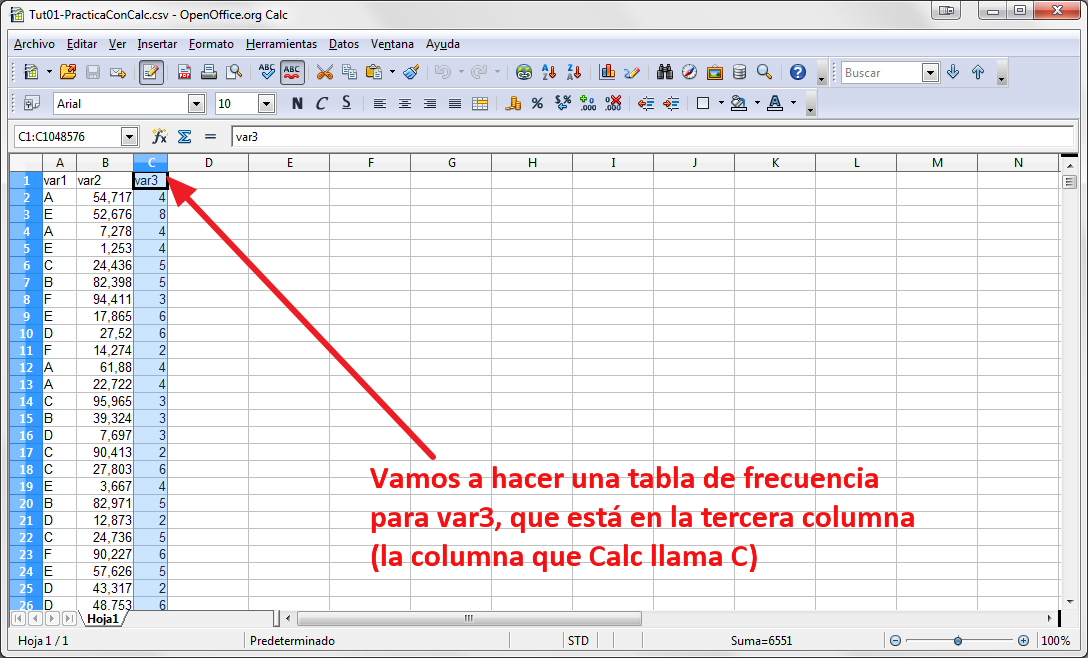
\includegraphics[height=8cm]{../fig/Tut01-Calc-tablaFrec-01.png}
    \end{center}
Si echamos un vistazo a los valores de esa columna veremos que se trata de números enteros. Pero es difícil saber, simplemente mirando, y teniendo en cuenta que hay 1300 filas, cuál es el valor máximo de esos números. Afortunadamente, Calc nos permite averiguar eso de una forma muy sencilla.
Vamos a utilizar una {\sf función} de la hoja de cálculo, la primera que encontramos. Veremos muchas más antes de que acabe el curso. La función que vamos a ver se llama {\tt MAX} y sirve para encontrar el valor máximo en un conjunto de celdas ocupadas por números.\\

{\bf Una advertencia:} en algunas versiones anteriores (pero recientes) de Calc, el nombre de esta función, y de algunas otras aparecía con acento, {\tt MÁX}. Y así lo verás en algunas figuras de este tutorial, que se prepararon con esas versiones previas. Asegúrate de cuál es el nombre correcto en la versión de Calc que estés utilizando.\\

Empezamos por situarnos en una celda no ocupada de la hoja de cálculo. Yo he usado la celda {\tt E4}, pero puedes usar otra celda libre. Por cierto, aprovechamos para indicar que las celdas de la hoja de cálculo se denotan así, con la letra de la columna seguida (sin espacio) del número de la fila, como en {\tt E4}. Haz clic en esa celda y asegúrate de que está seleccionada, como en esta figura:
    \begin{center}
    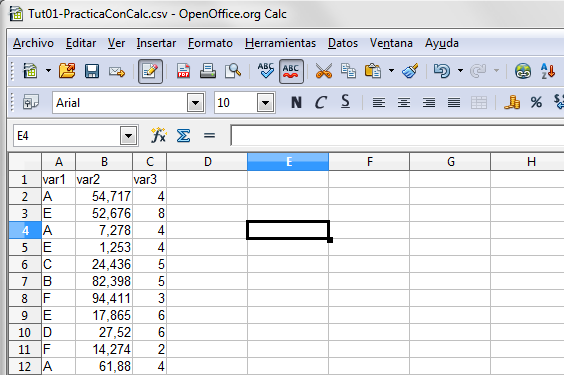
\includegraphics[height=8cm]{../fig/Tut01-Calc-tablaFrec-02.png}
    \end{center}
Ahora usa el menú {\tt Insertar} de Calc, y selecciona {\tt Función}
    \begin{center}
    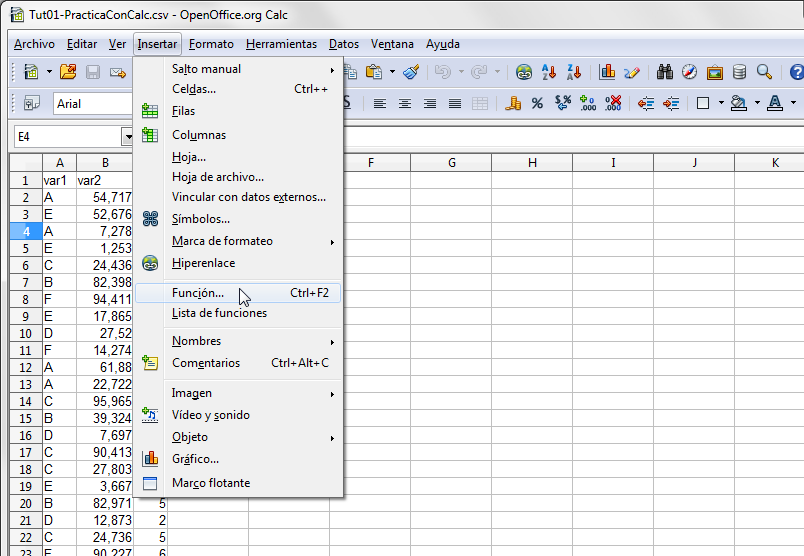
\includegraphics[height=8cm]{../fig/Tut01-Calc-tablaFrec-03.png}
    \end{center}
Aparecerá un cuadro de diálogo en el que tenemos que desplazarnos hacia abajo por la lista de funciones para buscar la función {\tt MAX}, como se ve en la siguiente figura:
    \begin{center}
    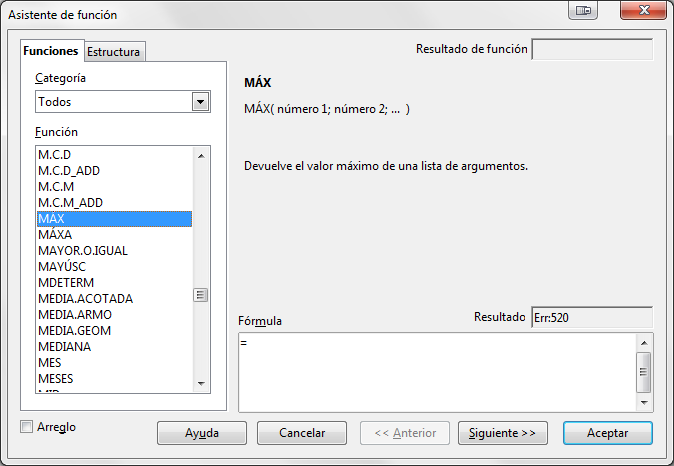
\includegraphics[height=8cm]{../fig/Tut01-Calc-tablaFrec-04.png}
    \end{center}
Una vez seleccionada esa función con un click, pulsamos en siguiente (o hacemos doble click en la función, es lo mismo). Aparece este diálogo, en el que debemos indicar cuáles son las celdas que contienen los números de los que queremos hallar el máximo. En nuestro caso, esas celdas están en la tercera columna, y van desde la {\tt C2} hasta la {\tt C1301}. Ten en cuenta, para entender esto, que la primera celda de esa columna, la {\tt C1},  está ocupada por el nombre de la variable. En Calc, para decir ``desde la celda {\tt C2} hasta la celda {\tt C1301}'' escribimos
    \begin{center}{\tt C2:C1301}\end{center}
separando los nombres de las dos celdas con dos puntos. Esto es lo que se llama un {\sf rango} de celdas (no hay que confundirlo con el {\em rango} o {\em recorrido} en sentido estadístico, del que se habla en la Sección \ref{curso-cap02:subsubsec:RangoIntercuartilico} del libro). Escribimos ese rango en el campo que se llama {\tt número 1} (no te preocupes de los otros, puedes dejarlos vacíos).
    \begin{center}
    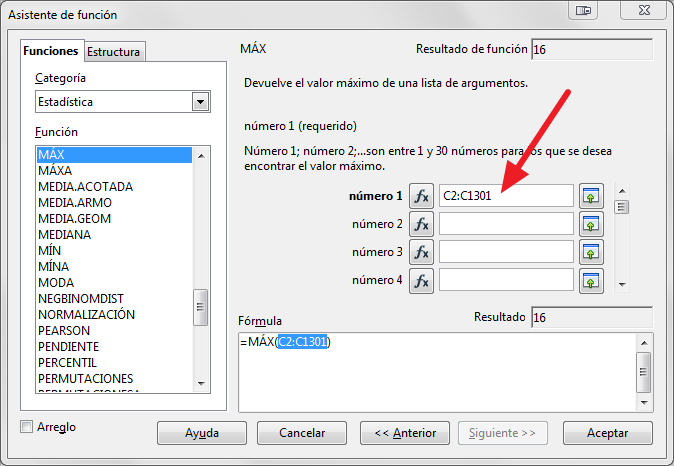
\includegraphics[height=10cm]{../fig/Tut01-Calc-tablaFrec-05.png}
    \end{center}
Fíjate también en el campo llamado {\em Resultado}, que muestra una vista previa del valor que vamos a obtener. Esta información es especialmente útil para detectar errores anticipadamente. \\

Ahora pulsamos en  {\tt Aceptar}, y el resultado aparece en la casilla que habíamos seleccionado.
    \begin{center}
    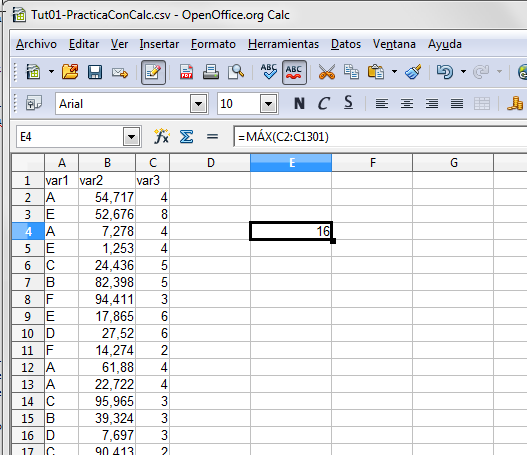
\includegraphics[height=9cm]{../fig/Tut01-Calc-tablaFrec-06.png}
    \end{center}
\subsection*{Pon a salvo tu trabajo. Ficheros binarios de tipo {\tt ods}.}
\label{tut01:subsec:PonASalvoTuTrabajo}

Antes de seguir adelante, vamos a hacer algo {\bf muy importante}, y a aprender la diferencia entre los ficheros {\tt csv} y otro tipo de ficheros, a los que llamaremos {\sf ficheros binarios}. Vamos a recordar donde estamos: hemos empezado con un fichero csv, lo hemos abierto en Calc, y ahora le hemos añadido una {\em ``operación con los datos''}, usando la función {\tt MAX}. Los ficheros {\tt csv} no sirven para almacenar ese tipo de operaciones, porque no están pensados para ello. Son ficheros muy simples, adecuados para {\em intercambiar} información, pero no para {\em procesarla}. Para almacenar las operaciones junto con los datos, tenemos que usar otro tipo de ficheros. Podemos seguir trabajando así un rato, pero si ocurre algo o nos equivocamos, perderemos todo el trabajo que llevemos hecho. Por eso vamos a guardar ahora nuestro trabajo, usando un formato de fichero que nos permita almacenar las operaciones.  Usamos el menú {\tt Archivo}, y seleccionamos {\tt Guardar como...}
    \begin{center}
    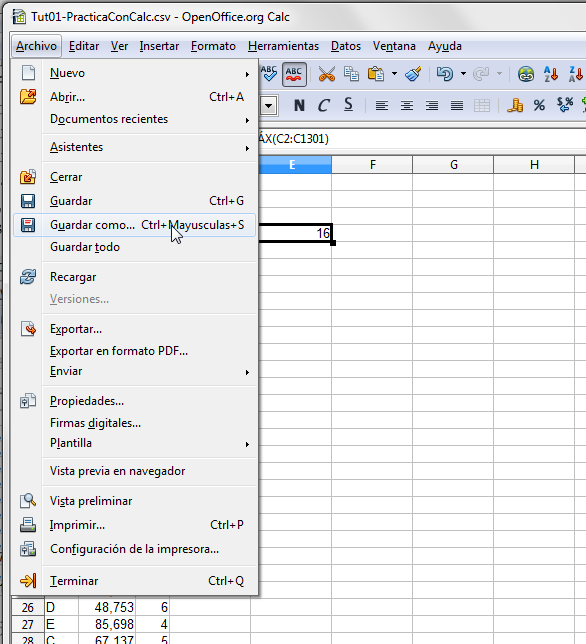
\includegraphics[height=9cm]{../fig/Tut01-Calc-tablaFrec-07.png}
    \end{center}
Aparecerá un cuadro de diálogo, como el que se ve en la siguiente figura,
    \begin{center}
    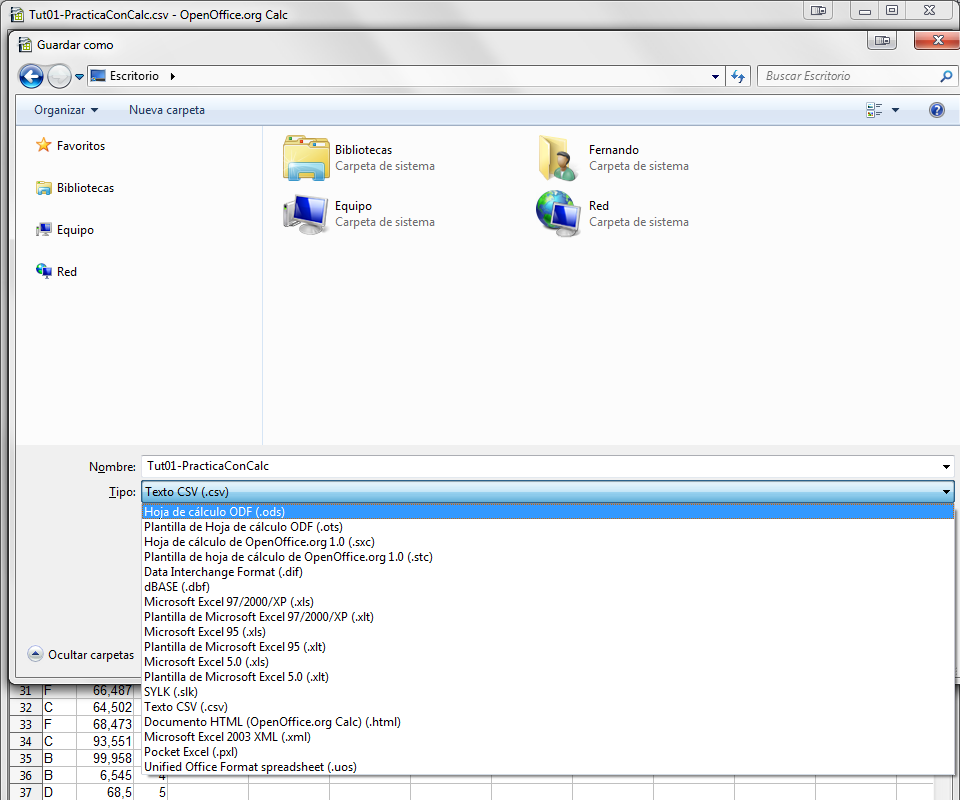
\includegraphics[height=8cm]{../fig/Tut01-Calc-tablaFrec-08.png}
    \end{center}
en el que debemos:
    \begin{enumerate}
    \item Elegir (y recordar) la carpeta en la que guardaremos el fichero. Recuerda que para los ficheros {\tt csv} usamos la subcarpeta {\tt datos} del {\em Directorio de Trabajo}.
    \item Elegir un nombre para el fichero. Vamos a usar
    \begin{center}
        {\tt Tut01-PracticaConCalc.ods}
    \end{center}
    Usa exactamente este nombre. No lo cambies, porque lo necesitarás en las próximas secciones.
    \item Seleccionar el tipo de archivo {\tt Hoja de cálculo ODF (.ods)}.
    \end{enumerate}
De esa forma, cuando pulsemos sobre el botón {\tt Aceptar} guardaremos datos y fórmulas en un mismo fichero, distinto del {\tt csv} con el que hemos empezado. En este paso puedes, si quieres, cambiar el nombre del fichero, aunque es recomendable que el nombre sea, si no igual, al menos parecido al del fichero {\tt csv} con el que hemos empezado. Lo que sin duda habrá cambiado es la {\sf extensión} del fichero, que habrá pasado de {\tt .csv} a {\tt .ods}. Estos ficheros {\tt ods} no son, desde luego, tan sencillos como los {\tt csv}. Es un ejercicio saludable abrir uno de ellos con el Bloc de Notas, por ejemplo este que acabamos de crear. Verás algo como esto:
    \begin{center}
    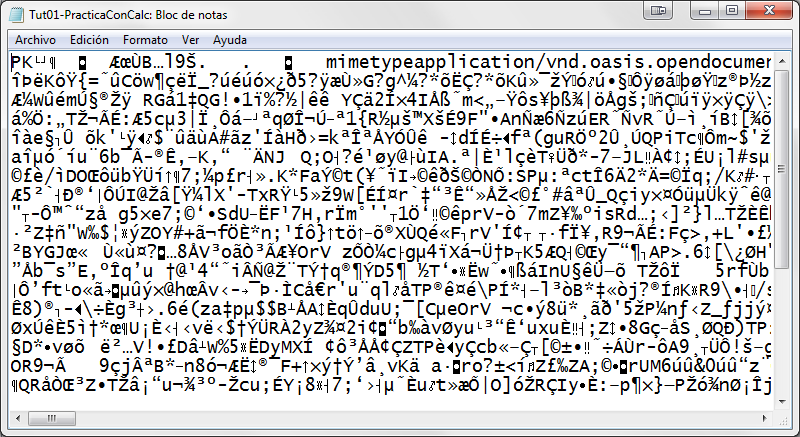
\includegraphics[height=8cm]{../fig/Tut01-Calc-tablaFrec-09.png}
    \end{center}
Es una jerigonza imcomprensible de código, en la que es básicamente imposible reconocer nuestros datos originales. La diferencia es que el {\tt csv} es un fichero de {\sf texto plano} (que también llamaremos un {\tt fichero fuente}), mientras que este {\tt ods} es un  {\sf fichero binario}. Simplificando un poco: los ficheros fuente los podemos escribir y entender las personas, mientras que los binarios están pensados para que los entienda el ordenador.

\subsection*{Obtener la tabla de frecuencias.}

Volvamos al trabajo de obtener la tabla de frecuencia de la variable {\tt var3}. Habíamos obtenido el valor máximo del rango {\tt C2:C1301}, que es 16, y lo habíamos guardado en la celda {\tt E4}.


%\stepcounter{EjercicioI}
%\paragraph{Ejercicio \theEjercicioI:}\quad\\
\begin{ejercicio}
\quad\\
Busca el valor mínimo de ese rango y guárdalo en la celda {\tt E5}.
\qed
\end{ejercicio}

\vspace{8cm}

\begin{center}
\textcolor{red}{\LARGE\bf  ¡No sigas, si no has hecho este ejercicio!}
\end{center}


\newpage

Como muestra la siguiente figura, deberías obtener un 0.
    \begin{center}
    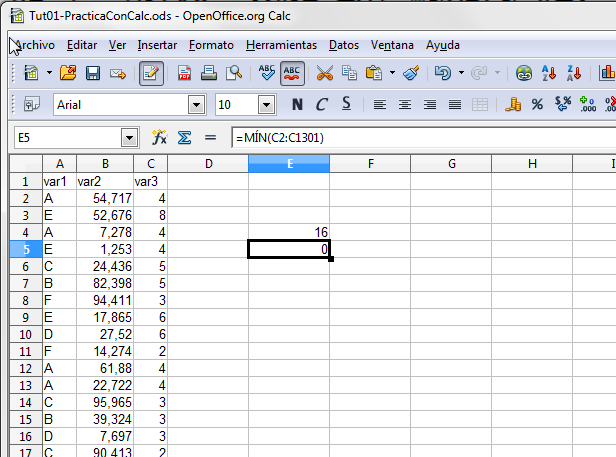
\includegraphics[height=9.3cm]{../fig/Tut01-Calc-tablaFrec-10.png}
    \end{center}
Ahora ya sabemos que ese rango contiene valores del 0 al 16. Asi que tenemos que obtener una tabla de frecuencias como esta:
\begin{center}
\begin{tabular}{|c|c|c|c|c|c|c|c|c|c|c|c|c|c|c|c|c|}
0&1&2&3&4&5&6&7&8&9&10&11&12&13&14&15&16\\
\hline
?&?&?&?&?&?&?&?&?&?&?&?&?&?&?&?&?
\end{tabular}
\end{center}

En Calc, vamos a obtener esta tabla en vertical, en la columnas {\tt G} y {\tt H} (puedes usar otras). Para ello, empieza por  colocar un 0 en la celda {\tt G2}:
    \begin{center}
    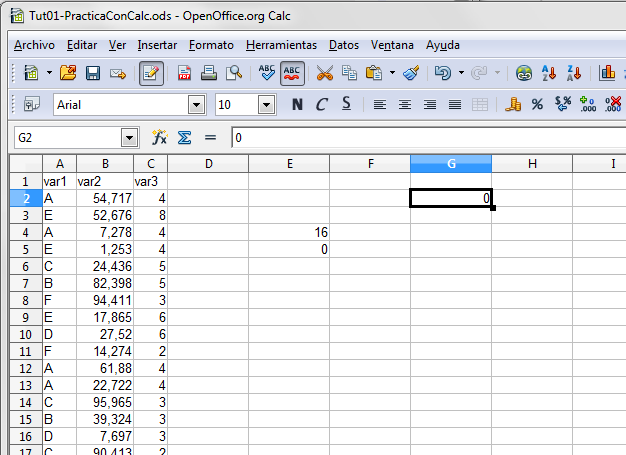
\includegraphics[height=9.3cm]{../fig/Tut01-Calc-tablaFrec-11.png}
    \end{center}
Ahora queremos colocar, en el rango de celdas {\tt G3:G18}, el resto de los números del 1 al 16, que forman la cabecera de la tabla de frecuencias. Si sabes algo sobre hojas de cálculo, sabrás que hay una forma muy rápida de hacer esto. Adelante, en ese caso. Si eres un recién llegado a este mundo, por el momento te toca escribir esos números ``a mano''. Pero no te preocupes, porque es la última vez que te lo pedimos: en la Sección \ref{tut01:sec:ComoTrabajarReferenciasHojasCalculo} de este tutorial te enseñaremos a ir mucho más rápido, y empezarás a entender cuál es el verdadero sentido y la utilidad de una hoja de cálculo como Calc.

\newpage

En cualquiera de los dos casos, suponemos que ahora el estado de la hoja de cálculo es este:
    \begin{center}
    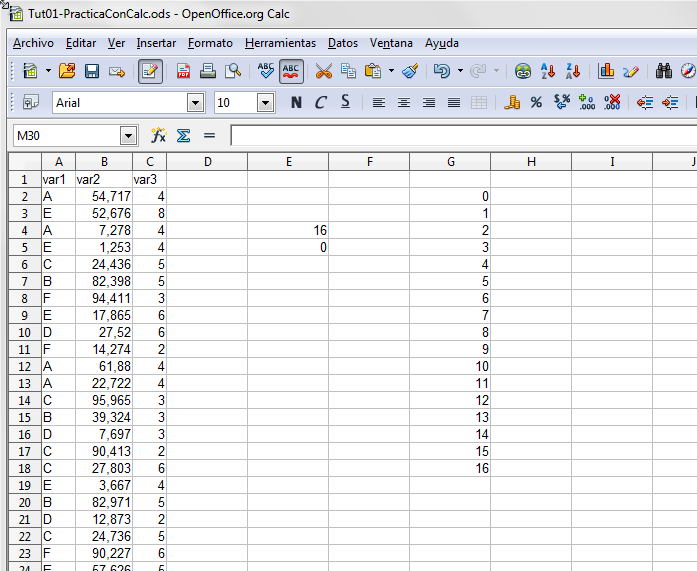
\includegraphics[height=10cm]{../fig/Tut01-Calc-tablaFrec-12.png}
    \end{center}
Y queremos que las frecuencias aparezcan justo a la derecha de estos valores, en el rango {\tt H2:H18}. El primer paso consiste en marcar ese rango, como en esta figura:
    \begin{center}
    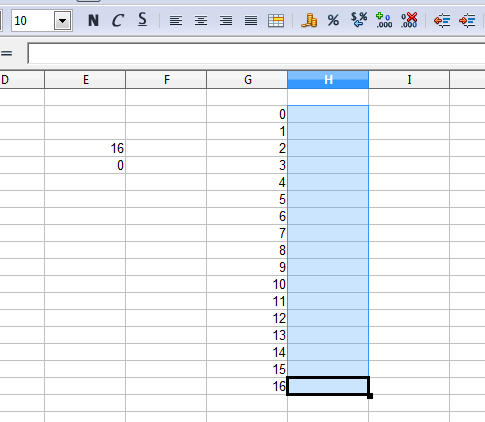
\includegraphics[height=8cm]{../fig/Tut01-Calc-tablaFrec-13.png}
    \end{center}
Es {\em muy importante} que todo el rango (y sólo el rango) esté marcado, exactamente como aparece en esa figura. Puesto que es la primera tabla de frecuencias que hacemos, lo vamos a hacer con mucho cuidado y saldrá bien. Pero en el futuro, cuando haya problemas, recuerda que la mayoría de los errores al obtener tablas de frecuencia con Calc se deben a que no se ha seleccionado correctamente el rango que ocupa la tabla.

A continuación vamos a utilizar una nueva función de Calc, que se llama, adecuadamente, {\tt FRECUENCIA}. Sin tocar nada (asegúrate de que el rango {\tt G2:G18} aparece marcado en azul) vamos al menú {\tt Insertar}, opción {\tt Función}, y en el cuadro de diálogo localizamos esa función {\tt FRECUENCIA}. Es conveniente que coloques ese cuadro de diálogo de forma que no cubra las columnas {\tt G} y {\tt H}, como verás que hemos hecho nosotros:
    \begin{center}
    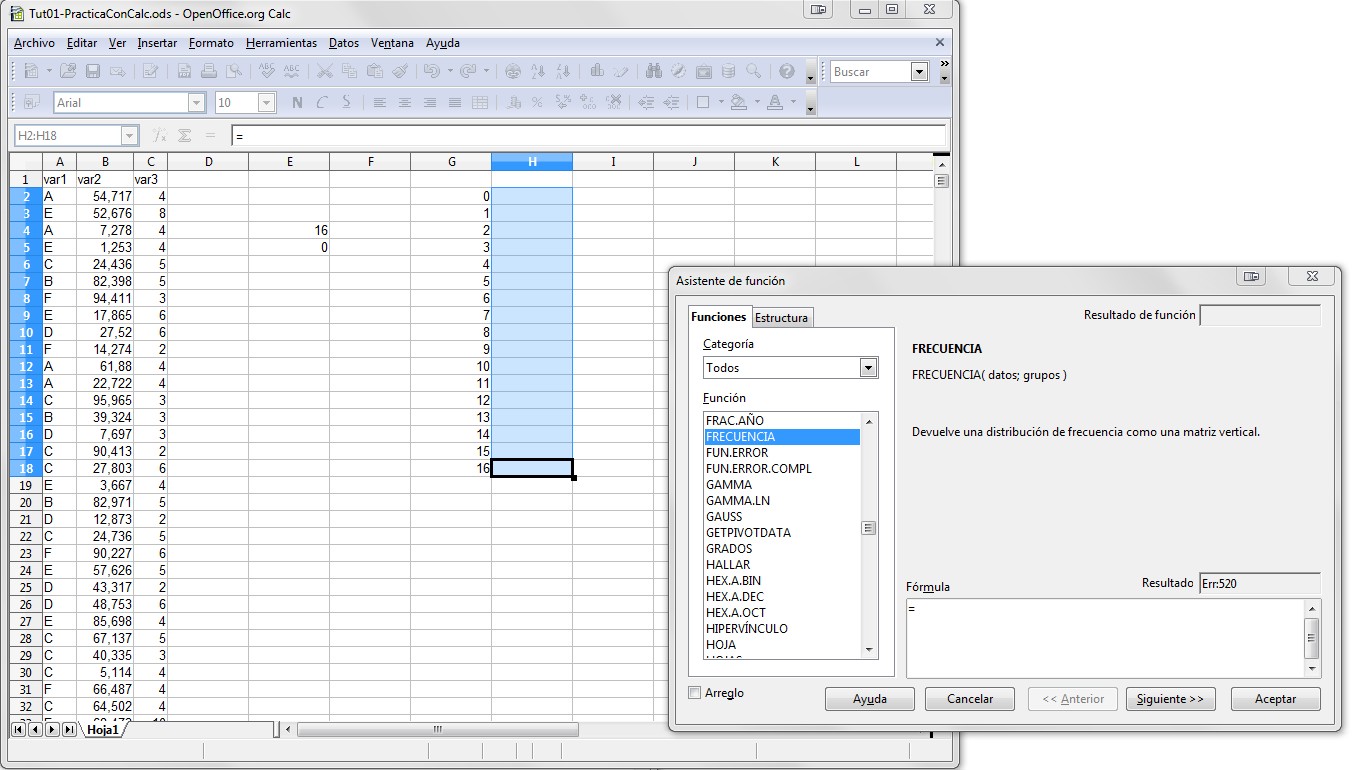
\includegraphics[height=9cm]{../fig/Tut01-Calc-tablaFrec-14.png}
    \end{center}
Pulsa en {\tt Siguiente} y asegúrate de rellenar los campos de este cuadro de diálogo de esta manera:
\begin{enumerate}
  \item En {\tt datos} indica los posiciones que ocupan los datos originales de {\tt var3}, es decir {\tt C2:C1301},
  \item En {\tt grupos} debes indicar las posiciones donde está la lista de valores distintos. O sea, la que será la primera columna de la tabla de frecuencias.  Es decir {\tt G2:G18}.
\end{enumerate}
También se pueden seleccionar esos rangos marcándolos con el ratón, y con la práctica, en muchos casos, decidirás si prefieres usar el ratón o el teclado. Haz experimentos, si quieres, y si algo no funciona, pulsa en {\tt Cancelar} y vuelve al paso anterior. En cualquier caso, al final debe quedar como en esta figura:
    \begin{center}
    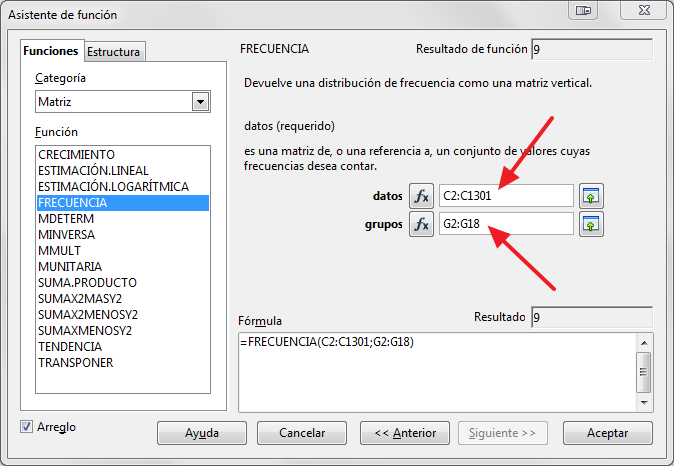
\includegraphics[height=9cm]{../fig/Tut01-Calc-tablaFrec-15.png}
    \end{center}
Ahora puedes pulsar en {\tt Aceptar} y verás aparecer tu nueva y flamante tabla de frecuencias:
    \begin{center}
    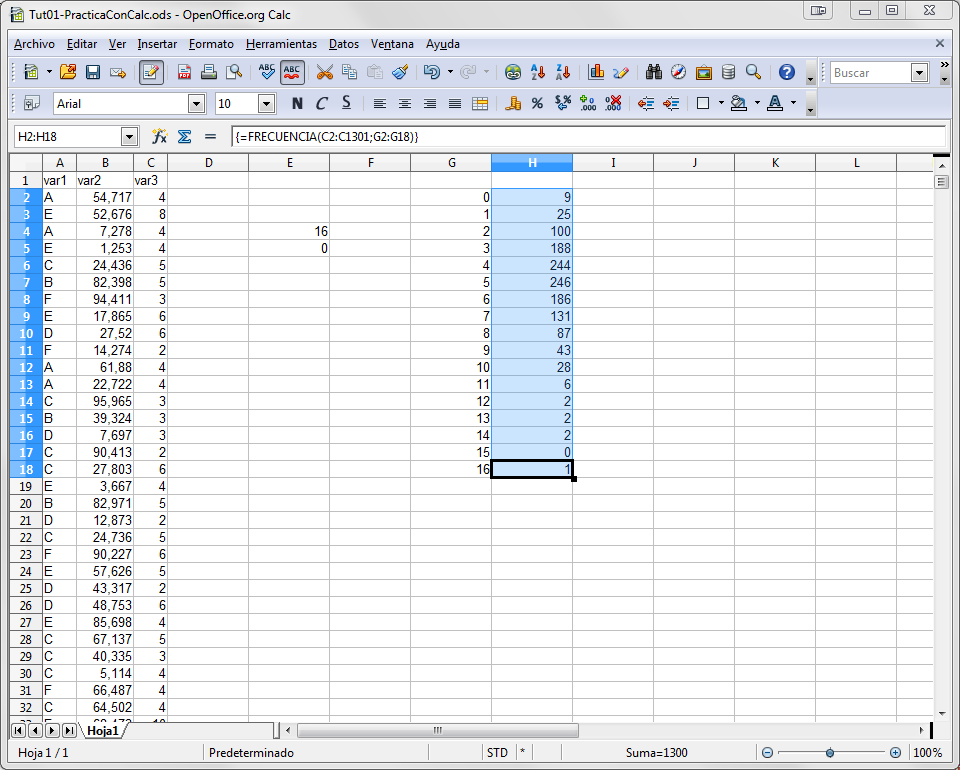
\includegraphics[width=16cm]{../fig/Tut01-Calc-tablaFrec-16.png}
    \end{center}
\paragraph*{}\label{tut01:lugar:TablaFrecuenciasVar3}¡Enhorabuena! Acabamos de dar el primer paso para convertirnos en gurús de la Estadística. Un vistazo rápido a la tabla que acabamos de obtener nos informa, por ejemplo, de que:
\begin{itemize}
  \item  el valor que más aparece es el 5, que se repite (su frecuencia es) 246 veces.
  \item  el valor 15 no aparece en la tabla (su frecuencia es 0).
  \item  la tabla de frecuencias tiene una ``forma'' curiosa, con valores que aumentan desde el 0 hasta el 5 y luego vuelven a disminuir.
\end{itemize}

\subsubsection*{Algunas observaciones adicionales.}
\label{tut01:subsubsec:ObservacionesAdicionalesTablasFrecuenciaSencillas}
\begin{itemize}
    \item En nuestro blog {\em PostData} hay una entrada, a la que puedes llegar con este enlace:
    {\scriptsize
    \begin{center}
    \link{http://fernandosansegundo.wordpress.com/2012/09/07/tablas-de-frecuencias-en-hojas-de-calculo-calc-y-excel}{
    http://fernandosansegundo.wordpress.com/2012/09/07/tablas-de-frecuencias-en-hojas-de-calculo-calc-y-excel} \end{center}
    }
    en la que se explica como hacer esto en la hoja de cálculo Excel. Es esencialmente igual, pero hay una pequeña diferencia al final del proceso, que te conviene conocer si vas a usar  Excel. Además, en esa entrada hay un vídeo que resume el proceso.

  \item No hemos hecho tablas de frecuencias de las variables {\tt var1} y {\tt var2} del fichero de datos {\tt Tut01-PracticaConCalc.csv}. La variable {\tt var1} nos obligaría a aprender algunos trucos sobre el uso de la hoja de Cálculo que no vamos a necesitar (porque usaremos programas más avanzados, como R), así que dejaremos ese asunto pendiente hasta más adelante (pero si te intriga, busca información sobre la función {\tt CONTAR.SI} de Calc). Por su parte, la variable {\tt var2} requiere agrupar los datos en clases, y nos va a llevar a aprender más sobre hojas de cálculo. Lo haremos en la Sección \ref{tut02:subsec:mediaAritmeticaDatosAgrupados}.
\end{itemize}
Pero antes, en la próxima sección, vamos a avanzar en nuestra comprensión del funcionamiento de las hojas de cálculo. \\

De momento, y para practicar lo que acabamos de aprender, vamos a hacer varios ejercicios.\\

\begin{ejercicio}
\label{tut01:ejercicio02}
\label{tut01:fichero:Tut01-PracticaConCalc-01}
En este ejercicio vamos a usar otro fichero de datos, que tienes aquí adjunto:
\begin{center}
\fichero{../datos/Tut01-PracticaConCalc-01.csv}{Tut01-PracticaConCalc-01.csv}.
\end{center}
%
% \\

Usando este fichero, haz lo siguiente:
\begin{enumerate}
  \item Abrelo con Calc, verás que contiene una única columna de datos, de una variable llamada {\tt x}. ¿Cuáles son sus valores mínimo y máximo?
  \item Antes de seguir, guarda tu trabajo en un fichero de tipo {\tt ods}, llamado
    \begin{center}
      {\tt Tut01-PracticaConCalc-01.ods}
    \end{center}
    ¡No lo olvides! Acostúmbrate a grabar los ficheros, de lo contrario puedes perder tu trabajo.  Además, vas a necesitar algunos de estos ficheros en futuros tutoriales.
  \item Construye la tabla de frecuencias de esa variable.
  \item ¿Cuál es el valor con mayor frecuencia? ¿Cuál el de menor? ¿Cuál es la frecuencia del valor 11?
  \item ¿Cuántos valores menores o iguales que 7 toma la variable {\tt x} (sumando todas las repeticiones que aparezcan en la columna {\tt A})?

\end{enumerate}
Tienes las soluciones al comienzo de la siguiente sección. Pero no te apresures a mirarlas, es imprescindible que aprendas a hacer estas operaciones antes de seguir.
\qed
\end{ejercicio}

\vspace{8cm}

\begin{center}
  \textcolor{red}{\LARGE\bf ¡No sigas, si no has hecho los ejercicios!}
\end{center}

\newpage
\section{Gráficos de barras y sectores.}

Para empezar a dibujar algunos gráficos con Calc, vamos a usar el fichero {\tt Tut01-PracticaConCalc-01.csv} (con el que has hecho el Ejercicio \ref{tut01:ejercicio02} del final de la sección anterior). Con este fichero vamos a aprender a dibujar gráficos de sectores y columnas en Calc. Pero antes, veamos la solución de ese ejercicio. Si todo ha ido bien, has debido obtener este resultado:
    \begin{center}
    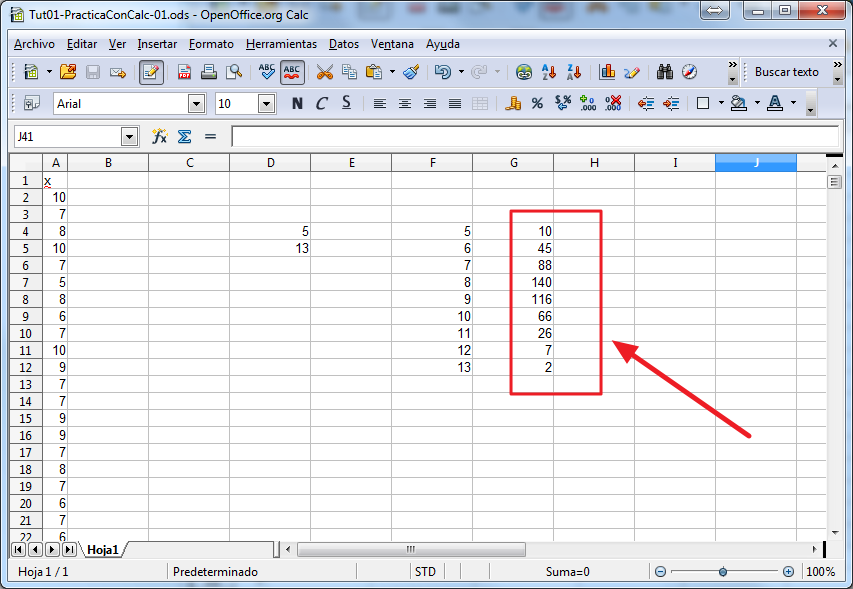
\includegraphics[height=11cm]{../fig/Tut01-Calc-Graficos-01.png}
    \end{center}
aunque es posible que hayas colocado los valores en otras celdas. Como ves, los valores mínimo y máximo de {\tt x} son, respectivamente, $5$ y $13$, el valor con mayor frecuencia es $8$ (su frec. es 140), el de menor frecuencia es 13 (su frec. es 2), y la frecuencia de 11 es 26. Para calcular cuántos valores menores que o iguales a $7$ toma {\tt x} tienes que sumar las frecuencias de 5,
6 y 7. Se obtiene:
\[10+45+88=143.\]

\paragraph{Gráfico de sectores.} Vamos a empezar dibujando uno de estos gráficos  que corresponda a la tabla de frecuencias que acabamos de obtener.
Seleccionamos toda la tabla,
    \begin{center}
    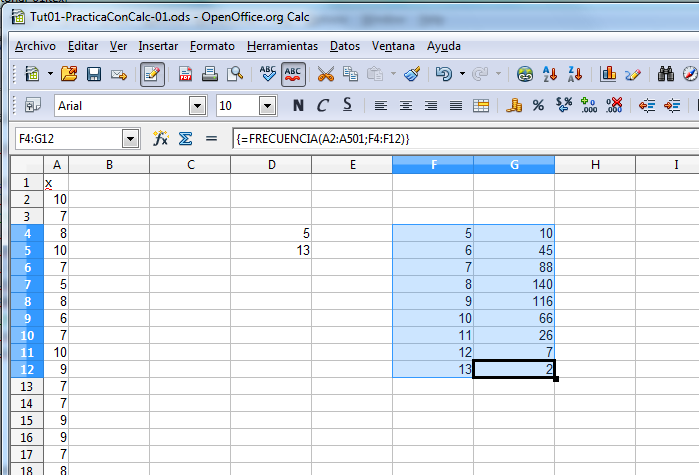
\includegraphics[height=8cm]{../fig/Tut01-Calc-Graficos-02.png}
    \end{center}
Y ahora vamos al menú {\tt Insertar}, opción {\tt Gráfico}. Aparecerá un gráfico y un cuadro de diálogo, como en la figura. No te preocupes por el gráfico, aún tenemos que ajustarlo.
    \begin{center}
    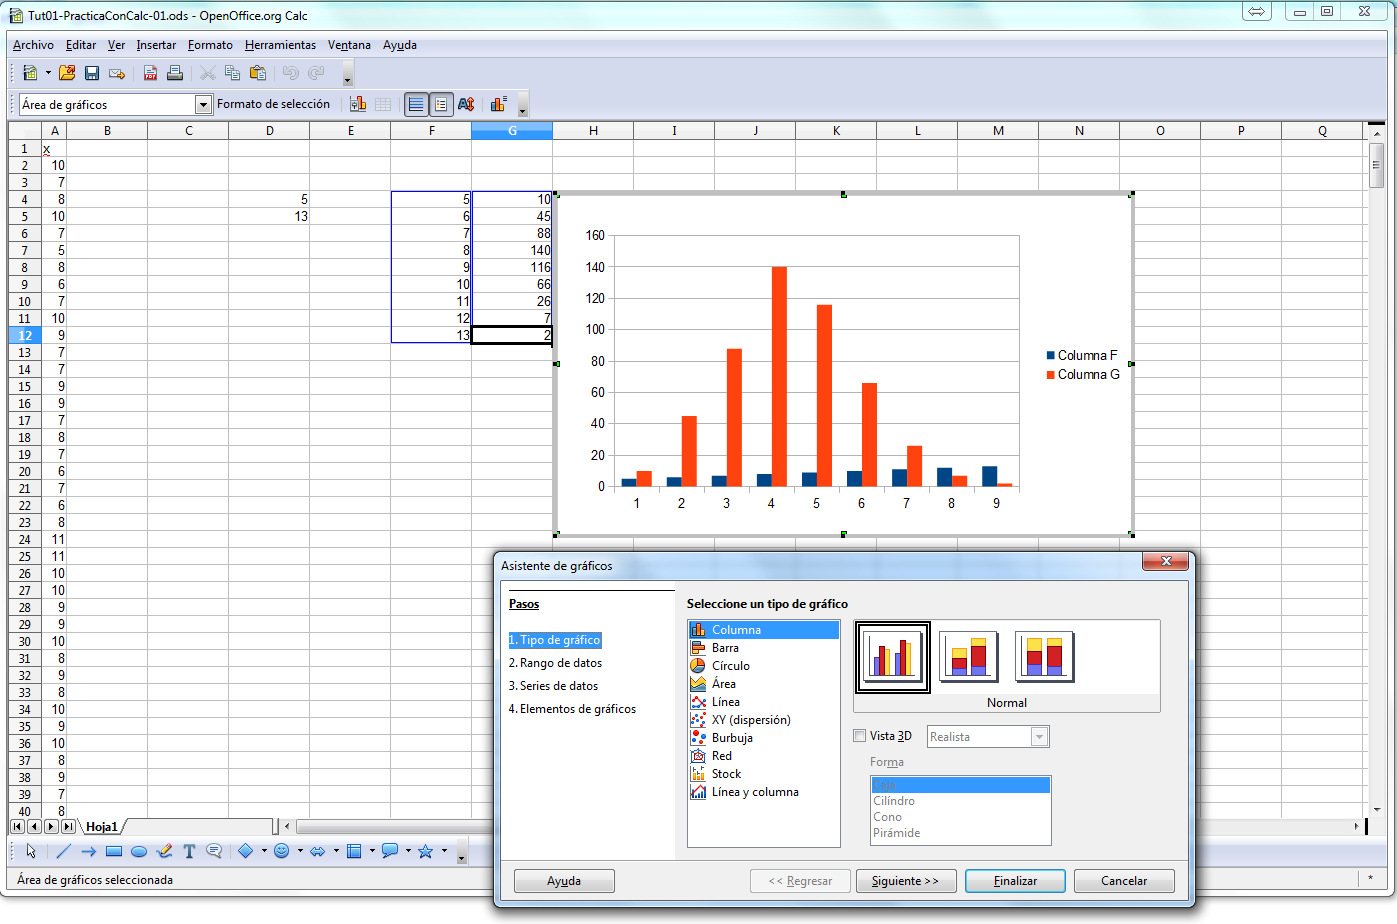
\includegraphics[height=11cm]{../fig/Tut01-Calc-Graficos-03.png}
    \end{center}
En ese cuadro de diálogo selecciona {\tt Círculo} y espera unos segundos.
    \begin{center}
    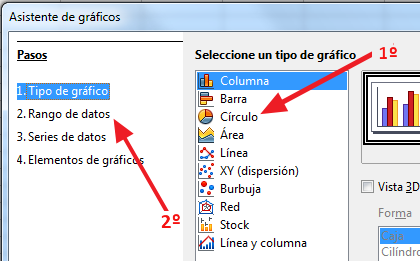
\includegraphics[height=7cm]{../fig/Tut01-Calc-Graficos-04.png}
    \end{center}
Verás aparecer un gráfico de sectores. ¡Pero es incorrecto, todavía debemos hacer otra cosa! En el cuadro de diálogo,
en la ventana de la izquierda, ve a {\tt 2. Rango de datos} y asegúrate de marcar la casilla de la opción {\tt Primera
columna como etiqueta.} Al hacerlo verás que el gráfico cambia. Al hacer esto le estamos pidiendo a Calc que interprete
las dos columnas de esa tabla como una tabla de valores y frecuencias.
    \begin{center}
    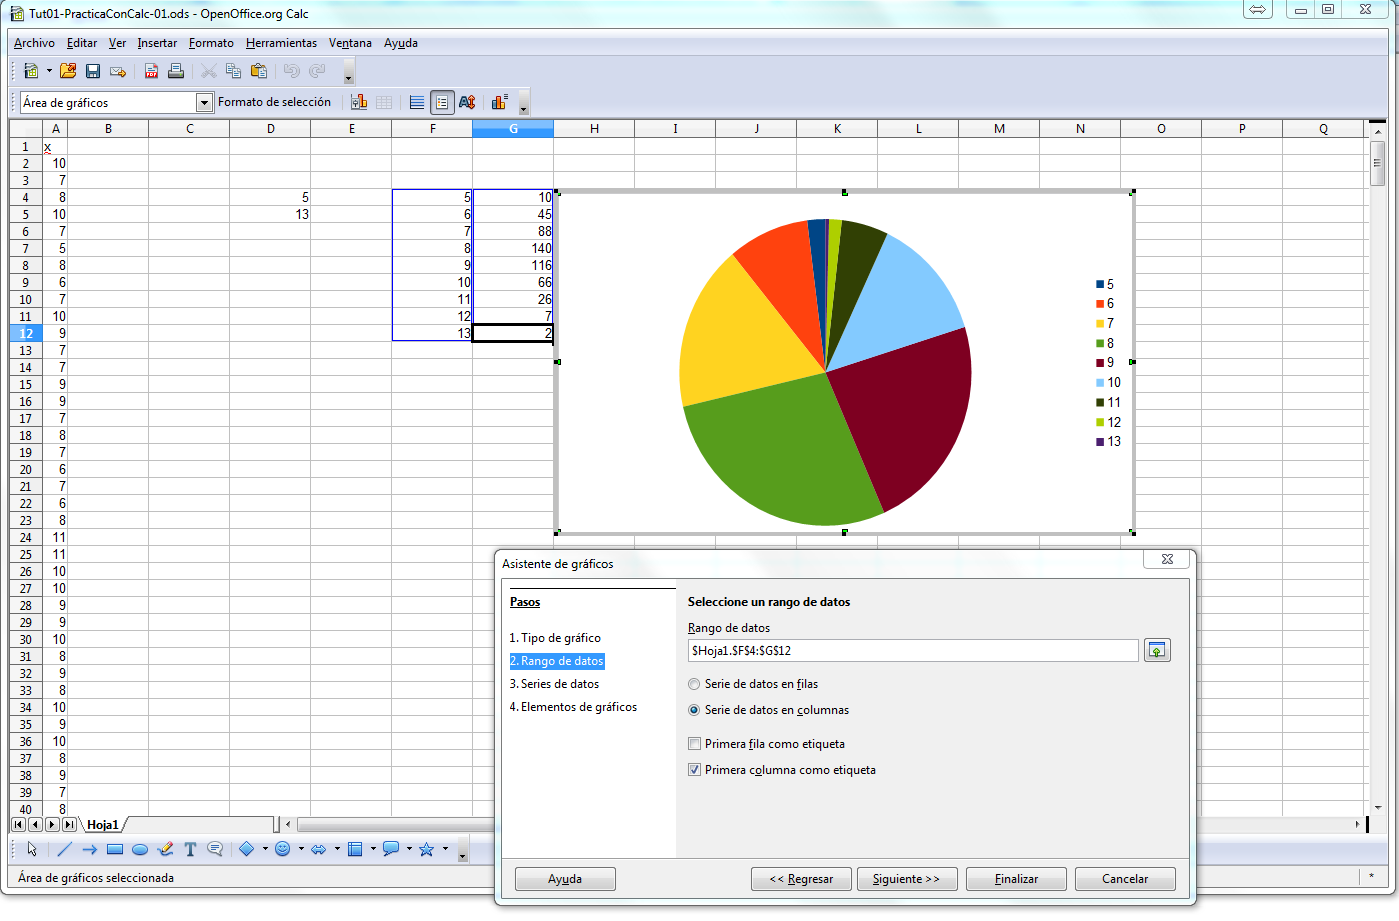
\includegraphics[height=9.5cm]{../fig/Tut01-Calc-Graficos-05.png}
    \end{center}
y ya puedes pulsar en {\tt Finalizar}. Puedes colocar ese gráfico dentro de la hoja de cálculo, donde más te convenga, pinchando sobre el pequeño marco gris que lo rodea y arrastrando con el ratón. No pinches en la zona blanca del gráfico (y si lo haces, usa {\tt Ctrl+Z} para deshacer.) También puedes copiar y pegar el gráfico si lo necesitas en otro documento.

\paragraph{Gráfico de barras.} Para terminar esta sección vamos a añadir un gráfico de barras (o columnas, la diferencia en todo caso es la orientación vertical u horizontal). El gráfico de sectores que hemos obtenido no es de los peores, pero en general desaconsejamos el uso de este tipo de gráficos. Queremos que entiendas cómo se hacen, y lo que significan, pero insistimos, demasiadas veces resultan confusos. Para obtener un gráfico de barras los pasos son muy parecidos. Vamos rápido: volvemos a seleccionar la tabla completa,
menú {\tt Insertar}, opción {\tt Gráfico}, pero ahora elegimos columnas, de nuevo en {\tt Rango de datos} marcamos la
casilla de {\tt Primera columna como etiqueta}, y veremos aparecer este gráfico:
    \begin{center}
    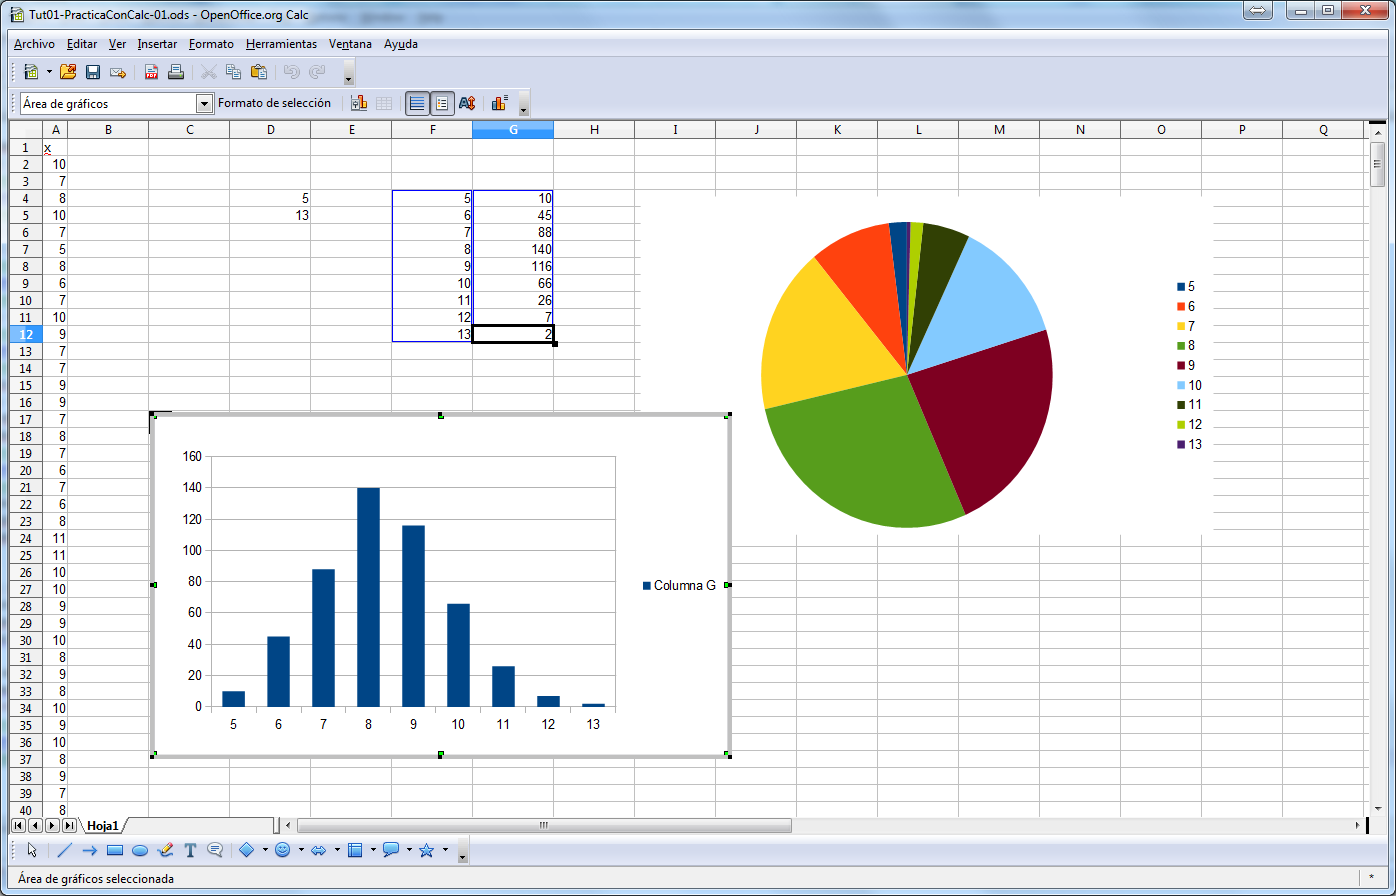
\includegraphics[height=9.5cm]{../fig/Tut01-Calc-Graficos-06.png}
    \end{center}
Los valores aparecen como etiquetas al pie de cada columna. Fíjate en lo fácil que resulta, en este gráfico, localizar los valores de mayor y menor frecuencia.

\begin{ejercicio}
\quad\\
Haz un gráfico de barras para la variable {\tt var3} del fichero {\tt Tut01-PracticaConCalc.csv}, que encontrarás adjunto en la página \pageref{tut01:sec:TablasFrecuenciaSencillas}.
\qed
\end{ejercicio}

En ese mismo fichero, la representación gráfica adecuada para la variable {\tt var2}, una vez agrupada en clases, es un histograma. Todavía no hemos aprendido a agrupar por clases en Calc. Y, en cualquier caso, con Calc no es fácil dibujar histogramas correctamente. Pero no hay que preocuparse. En el próximo tutorial empezaremos a usar R, la herramienta a la que más tiempo vamos a dedicar, y veremos que con R, dibujar histogramas es muy fácil.


\section{Cómo usar las referencias a celdas de la hoja de cálculo.}
\label{tut01:sec:ComoTrabajarReferenciasHojasCalculo}

Este apartado va dirigido a aquellos lectores que tienen escasa o nula experiencia con una hoja de cálculo como Calc o Excel. Para ellos, es obligatorio una lectura atenta de lo que sigue, y además es necesario ir reproduciendo simultáneamente todos los pasos en un ordenador. Si te atascas en alguno de ellos, vuelve a leer, asegúrate de que estás haciendo exactamente lo que se describe en el texto. Y si aún así tienes problemas, pide ayuda a quien sepa más que tú \ninja{(ya sabes...).} Si, por el contrario, te mueves con soltura en este tipo de programas, seguramente no vas a aprender nada nuevo. Aún así te recomendamos, al menos, una lectura rápida para comprobar que no hay sorpresas, y para que te familiarices con la terminología que vamos a usar. Después, puedes pasar directamente al siguiente apartado.

En la Sección \ref{tut01:sec:TablasFrecuenciaSencillas}, al construir la tabla de frecuencias para la variable {\tt var3},  teníamos que rellenar una rango de celdas de Calc con los números del 1 al 16. Y dijimos entonces que había una forma rápida de hacer esto, que vamos a ver a continuación. Empieza por abrir de nuevo con Calc el fichero {\tt Tut01-PracticaConCalc.csv} (lo tienes en la página \pageref{tut01:sec:TablasFrecuenciaSencillas} de este tutorial), recordando los pasos necesarios para esa tarea. Si lo tienes a mano, también puedes usar el fichero de tipo {\tt ods}, pero te recomendamos empezar a partir del {\tt csv}.

Vamos a suponer, para empezar, que Calc está abierto, el fichero se ha cargado, y estamos en este estado:
    \begin{center}
    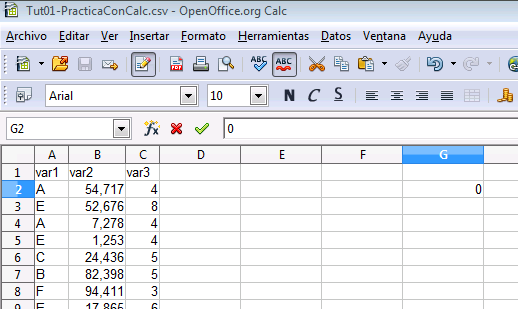
\includegraphics[height=8cm]{../fig/Tut01-Calc-Formula-00.png}
    \end{center}
de manera que la celda {\tt G2} contiene el número 0. Recuerda, {\tt G2} significa: columna {\tt G} y fila {\tt 2}. Nuestro objetivo es que aparezcan los números 1 al 16 en las celdas {\tt G3:G18} (recuerda que los dos puntos indican un {\sf rango} o grupo de celdas contiguas en la hoja de cálculo). Vamos a ir paso a paso, en el futuro podrás ir más rápido. La idea básica es que:
\begin{center}
{\em el contenido de cada celda se obtiene sumando 1 al de la celda que tiene encima.}
\end{center}
La propiedad más importante de una hoja de cálculo es que es muy fácil utilizar descripciones como {\em ``la celda que está encima''} o {\em ``la celda situada dos posiciones hacia la derecha''}, etcétera. Y además, esas descripciones se pueden {\em copiar y pegar}, también muy fácilmente. No te preocupes si ahora mismo todo esto parece un poco confuso, con la práctica lo verás claro.

Ahora,  haz clic con el ratón sobre la celda {\tt G3}, y pulsa la tecla {\tt =}. Al usar esta tecla le estamos diciendo a Calc que esa celda va a contener una {\sf fórmula}, algo que la hoja de cálculo va a tener que calcular, en lugar de simplemente un valor que nosotros tecleamos directamente.  A continuación del símbolo igual, teclea {\tt G2+1}, como se ve en la figura. Esa es la expresión de la fórmula que Calc tiene que calcular. Y significa, como es fácil imaginar, ``toma el contenido de {\tt G2} y súmale 1''.
    \begin{center}
    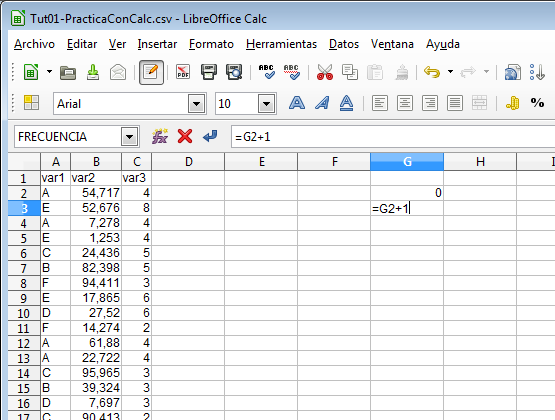
\includegraphics[height=10cm]{../fig/Tut01-Calc-Formula-01.png}
    \end{center}
Cuando pulses {\tt Entrar}, en la casilla {\tt G3} aparecerá un 1. Pero si haces clic sobre esa casilla, y miras en la {\em Línea de Entrada} (indicada por la flecha roja de la figura), verás la fórmula que hemos utilizado.
    \begin{center}
    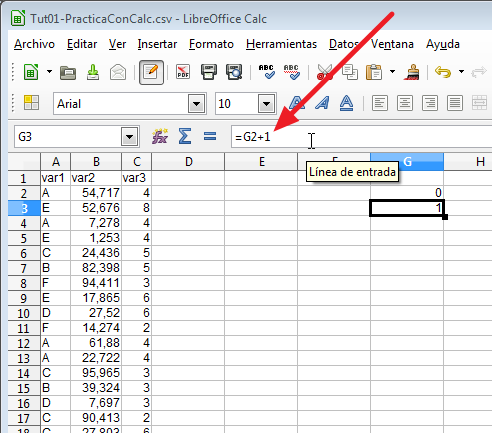
\includegraphics[height=10cm]{../fig/Tut01-Calc-Formula-02.png}
    \end{center}
Hasta aquí, seguramente, no hemos hecho nada demasiado espectacular. Ahora empieza lo bueno: asegúrate de tener seleccionada la celda {\tt G3} (aparecerá resaltada, con un rectángulo negro más grueso). Vamos a copiar esa celda al Portapapeles. Puedes pulsar {\tt Ctrl+C}, o usar el botón derecho del ratón como muestra la figura
    \begin{center}
    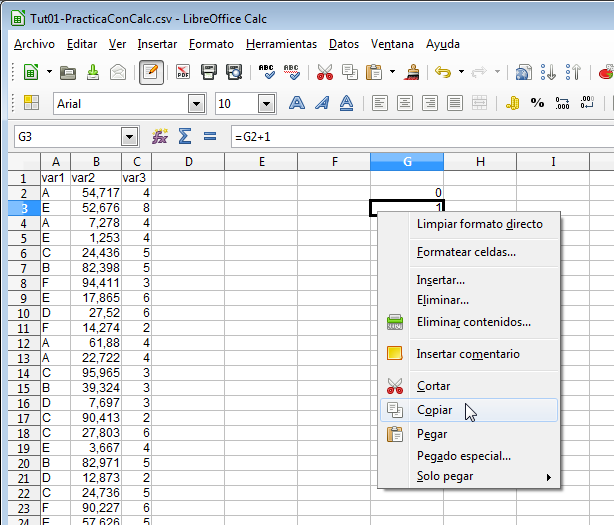
\includegraphics[height=10cm]{../fig/Tut01-Calc-Formula-03.png}
    \end{center}
Al hacerlo puede que veas que la celda {\tt G3} queda doblemente resaltada, con una línea de trazos (depende de la versión de Calc que uses). Ahora haz clic en la celda {\tt G4} y, manteniendo pulsado el ratón, arrástralo para marcar (seleccionar) las restantes celdas del rango, de la {\tt G4} a la {\tt G18}. Si se hace correctamente, las celdas quedarán marcadas en azul, como en esta figura:
    \begin{center}
    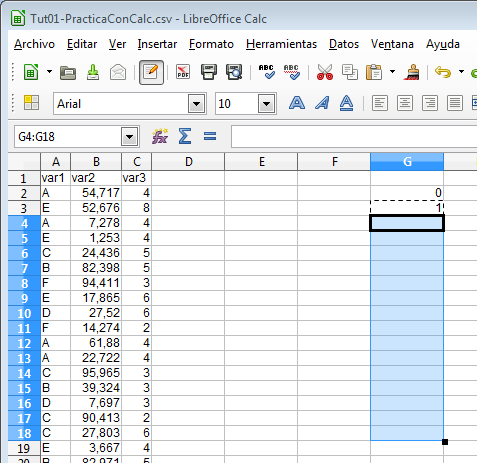
\includegraphics[height=11cm]{../fig/Tut01-Calc-Formula-04.png}
    \end{center}
Ahora vamos a pegar en esas celdas la fórmula que hemos copiado al Portapapeles, Para ello puedes pulsar {\tt Ctrl+V}, o puedes de nuevo usar el botón derecho del ratón (y seleccionar {\tt Pegar}, claro). El resultado será la lista de números que queríamos:
    \begin{center}
    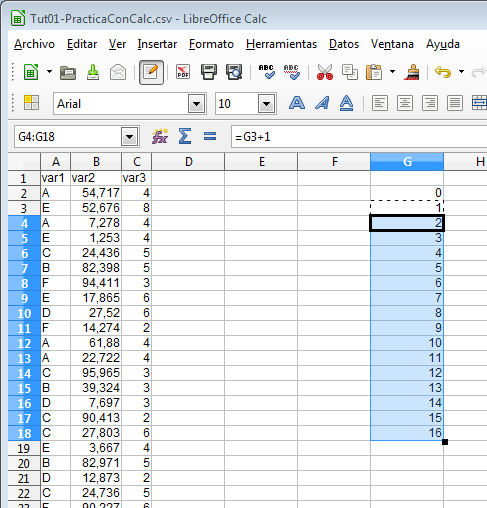
\includegraphics[height=11cm]{../fig/Tut01-Calc-Formula-05.png}
    \end{center}
Para entender mejor lo que ha sucedido, haz clic con el ratón en una de las celdas del rango (yo he usado la {\tt G13}) y mira en la {\em Línea de Entrada}, para ver la fórmula que Calc está utilizando. Verás que allí aparece {\tt =G12 + 1}. Lo que Calc hace, cuando copia una fórmula, es copiar la descripción de la fórmula en términos de posiciones {\sf relativas} y no {\sf absolutas}. Es decir, que al usar descripciones como ``la celda de arriba'', si estamos en {\tt G13} eso significa la celda {\tt G12}, y si estuviéramos en {\tt E7} significaría {\tt E6}. Este tipo de descripciones relativas es lo que hace que sea muy fácil manejar y operar con rangos de celdas en la hoja de cálculo, para repetir operaciones con todos los datos de un conjunto. Más adelante en esta sesión, veremos que hay ocasiones en que, precisamente, lo que necesitamos es usar una posición absoluta, y veremos cómo se hace esto.

\subsubsection*{Deshacer operaciones}
\label{tut01:subsubsec:DeshacerOperaciones}

Antes de seguir adelante, vamos a aprender a deshacer operaciones; esto será muy útil si cometemos algún error, para evitarnos tener que retroceder hasta el principio. En la barra de herramientas de Calc verás un par de símbolos en forma de flechas curvadas, llamados respectivamente {\em deshacer} y {\em rehacer}.
    \begin{center}
    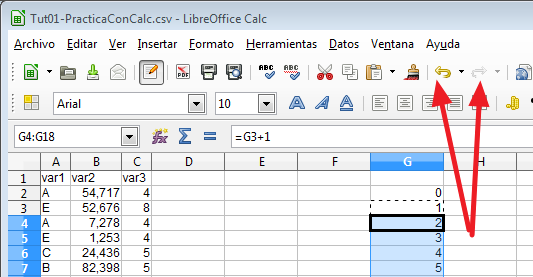
\includegraphics[height=7cm]{../fig/Tut01-Calc-Formula-06.png}
    \end{center}
Pulsa el símbolo de deshacer y verás desaparecer la lista de números que obtuvimos en el último paso. Si vuelves a pulsarlo Calc deshace la anterior operación que hicimos, y así sucesivamente. Haz clic unas cuantas veces sobre ese símbolo, y luego haz clic sobre el símbolo {\em rehacer}, hasta que hayas entendido como funcionan. Si eres más amigo del teclado, puedes usar {\tt Ctrl+Z} y {\tt Ctrl+Y} en lugar de deshacer y rehacer, respectivamente. Estas combinaciones de teclas funcionan en muchos otros programas, además de Calc, así que es bueno que las conozcas.

Usa estas dos herramientas para volver a la situación en la que sólo estaban ocupadas las celdas {\tt G2} (con un 0) y {\tt G3} (con un 1, resultado de la fórmula {\tt =G2+1}). Ahora podemos seguir adelante.

\subsubsection*{Otra manera de copiar las fórmulas}
Haz clic en {\tt G3} y fíjate en que la esquina inferior derecha de esa celda aparece un pequeño cuadrado negro. Haz clic sobre ese cuadrado, y manteniendo el botón izquierdo del ratón pulsado, arrastralo para cubrir el resto del rango {\tt G3:G18}. Si lo haces correctamente, mientras arrastras verás que esas celdas van quedado enmarcadas por un rectángulo rojo. En la figura puedes ver un momento intermedio del proceso:
    \begin{center}
    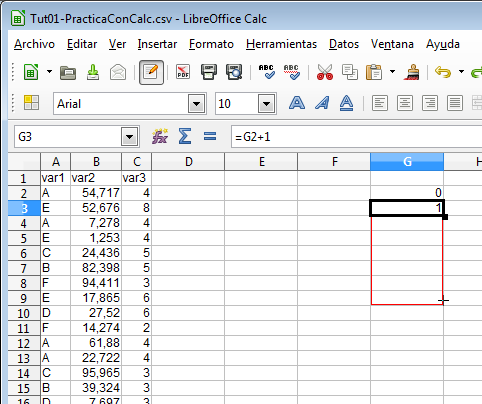
\includegraphics[height=8cm]{../fig/Tut01-Calc-Formula-07.png}
    \end{center}
Al llegar a {\tt G18} libera el ratón, y verás que aparecen de nuevo los números del 2 al 16 en esas aceldas. Este procedimiento de arrastrar es útil para copiar una fórmula rápidamente a un pequeño rango de celdas.

Si quieres guardar el trabajo que has hecho en esta hoja, recuerda que debes hacerlo en formato {\tt ods}, y no en formato {\tt csv}. Es importante entender que el formato {\tt ods} es capaz de almacenar fórmulas y gráficos, mientras que el {\tt csv} sólo almacena los datos. Es bueno, para practicar esto, que después del trabajo de esta sección guardes el fichero en los dos formatos, con nombres distintos si es preciso, y que después los abras para ver las diferencias. En cualquier caso, si tratas de guardar un fichero que contiene fórmulas o gráficos en formato {\tt csv}, Calc te avisará con un mensaje de advertencia
    \begin{center}
    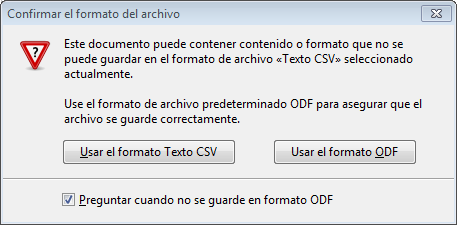
\includegraphics[height=4cm]{../fig/Tut01-Calc-Formula-08.png}
    \end{center}

\subsubsection*{Números (pesudo)aleatorios con Calc}
\label{tut01:subsubsec:NumerosAleatoriosCalc}

Para aprender algo nuevo, y practicar un poco más con el manejo de fórmulas, vamos a usar otra función de Calc. A lo largo del curso vamos a necesitar muchas veces hacer experimentos con datos elegidos ``al azar''. Tendremos sobradas ocasiones de discutir en detalle lo que queremos decir con esto, pero  por el momento puedes pensar que es como si lanzáramos un dado muchas veces y  fuéramos anotando los resultados. Naturalmente, un ordenador no es un dado, y no se pueden fabricar números verdaderamente aleatorios usando un programa de ordenador. Pero se pueden obtener números {\sf pseudoaleatorios}, que son más que suficientes para nuestros propósitos. Veamos cómo hacerlo con Calc. Abrimos una hoja de cálculo nueva (Menú {\tt Archivo} $\to$ {\tt Nuevo} $\to${\tt Hoja de cálculo}, o simplemente {\tt Ctrl+N}).

Vamos a usar el rango {\tt A1:A100} para simular 100 lanzamientos de un dado. Para conseguir esto vamos a usar una función de Calc, como las funciones {\tt MIN}, {\tt MAX} y {\tt FRECUENCIA} que ya hemos visto. La función que necesitamos ahora se llama {\tt ALEATORIO.ENTRE} (en inglés es {\tt RANDBETWEEN}).  Esta función sirve para obtener un número entero aleatorio entre dos valores que elegimos nosotros. Podríamos usar el menú {\tt Insertar} $\to$ {\tt Función}, como aprendimos a hacer, pero vamos a hacerlo de otra manera para ver que el resultado es el mismo (dejamos para el lector la tarea de comprobar el uso de los menús).

Empezamos haciendo click, por ejemplo, en la celda {\tt A1}. Y ahora tecleamos:
\begin{center}
{\tt =ALEATORIO.ENTRE(}
\end{center}
Da igual que uses mayúsculas o minúsculas, pero tienes que empezar con el {\tt =} (que le dice a Calc que a continuación viene una fórmula) y abrir un paréntesis al final. Justo después de escribir el paréntesis verás aparecer un mensaje que indica que Calc ha reconocido la función que estamos usando, y nos da alguna pista sobre la forma correcta de usarla:
    \begin{center}
    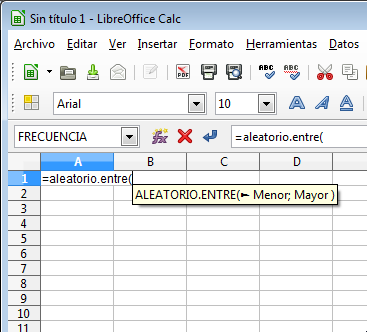
\includegraphics[height=8cm]{../fig/Tut01-Calc-Formula-09.png}
    \end{center}
En particular, esta función necesita dos números, sus {\sf argumentos}, que Calc representa como {\tt Menor} y {\tt Mayor}. En el caso de un dado, usaremos 1 y 6 como valores {\tt Menor} y {\tt Mayor}, respectivamente. Así que terminamos de escribir la función  son esos valores, separados por punto y coma. ¡Esto es importante! En las hojas de cálculo los rangos se indican con dos puntos, como sabemos, y los argumentos de funciones se separan con punto y coma. Muchos de los errores que se cometen se deben a confundir cosas como estas. Una vez tecleado esto:
    \begin{center}
    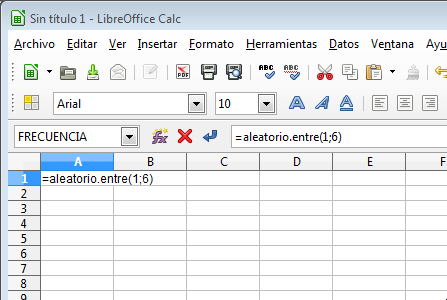
\includegraphics[height=7cm]{../fig/Tut01-Calc-Formula-10.png}
    \end{center}
pulsamos {\tt Entrar}, y obtenemos algo como esto:
    \begin{center}
    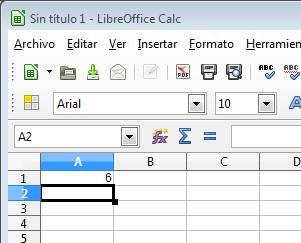
\includegraphics[height=5cm]{../fig/Tut01-Calc-Formula-11.png}
    \end{center}
¡Atención! Si lo haces en tu ordenador, obtendrás probablemente otro número del uno al seis. Al fin y al cabo de eso se trata. Estamos simulando el lanzamiento de un dado, y es como si tú lanzaras un dado y yo otro.

Ahora queremos repetir esto cien veces. Y evidentemente, no se trata de que repitas los pasos anteriores cien veces en cada una de las casillas {\tt A2:A100}. No, lo que vamos a hacer es copiar la fórmula de {\tt A1}, como hemos aprendido a hacer. Hay varias formas de hacer esto. Mira la figura, que te da una pista del procedimiento que hemos usado nosotros.
    \begin{center}
    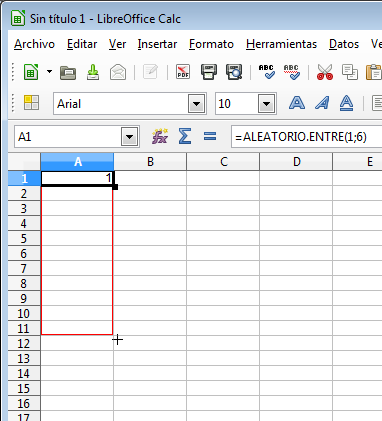
\includegraphics[height=7cm]{../fig/Tut01-Calc-Formula-12.png}
    \end{center}
El resultado final es una colección de cien números del uno al seis, de la que aquí mostramos el final (los tuyos serán distintos, claro).
    \begin{center}
    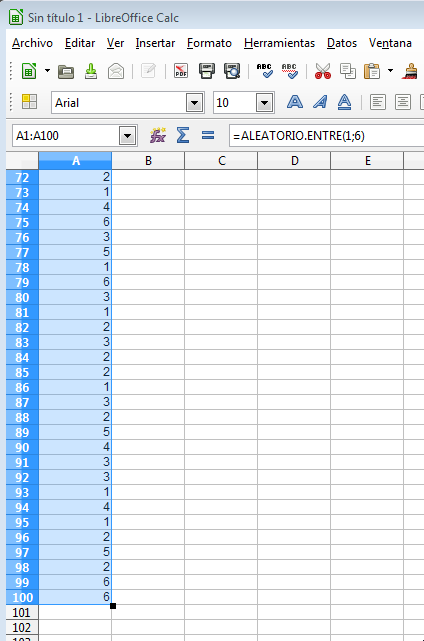
\includegraphics[height=8cm]{../fig/Tut01-Calc-Formula-13.png}
    \end{center}
Si guardas el fichero (en formato {\tt ods}, claro), cada vez que lo abras Calc volverá a calcular esos números aleatorios y obtendrás cien distintos cada vez (¿Cuánta suerte crees que necesitas para que te salgan dos veces los mismos cien números?
% Calcular 6^100/(3600*24*365*100) para ver cuantas 'vidas' lanzando 100 dados cada segundo es esto.
Más adelante en el curso contestaremos...) Si quieres volver a calcular los números sin tener que cerrar y abrir Calc, prueba a pulsar simultáneamente {\tt Ctrl + Mays + F9}.


\section{Media aritmética.}
\label{tut01:sec:mediaAritmeticaHojaCalculo}

En esta sección, y en las siguientes, vamos a empezar a usar las características de la hoja de cálculo para explorar los conceptos que se discuten en el Capítulo \ref{curso-cap:ValoresCentralesDispersion} del libro. Empezaremos con la media aritmética, analizando como calcularla según la situación de partida.

\subsection{El caso de valores no agrupados.}
\label{tut01:subsec:MediaAritmeticaCalculoDirecto}

El fichero adjunto
\begin{center}
\fichero{../datos/Tut01-mediaAritmeticaConCalc.csv}{Tut01-mediaAritmeticaConCalc.csv}
\end{center}
contiene treinta valores de los que queremos calcular la media aritmética. Empieza por abrir el fichero con Calc.  Al hacerlo, debes ver esto en tu pantalla:
    \begin{center}
    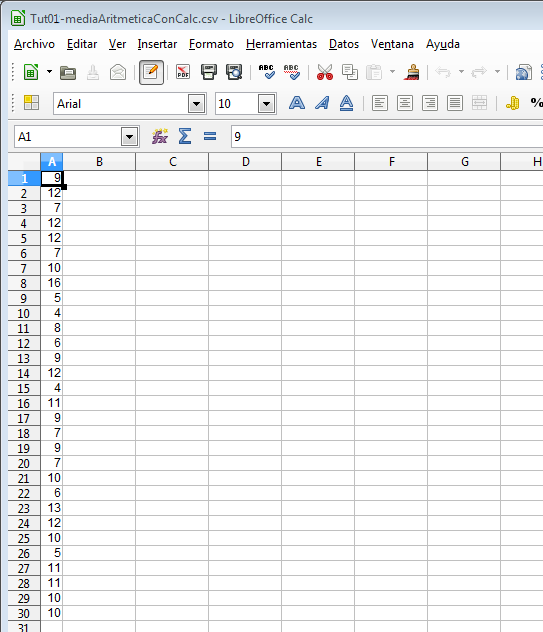
\includegraphics[height=11cm]{../fig/Tut01-Calc-Formula-14.png}
    \end{center}
Vamos a calcular la media aritmética de estos números, y lo haremos de varias maneras. Empezamos recordando la definición, que es:
   \[\bar x=\dfrac{x_1+\cdots+x_n}{n}=\dfrac{\displaystyle\sum_{i=1}^nx_i}{n}.\]
Así que la receta dice que tenemos que:
\begin{enumerate}
  \item sumar todos los números
  \item y dividir el resultado por $n$, que es la cantidad de números que tenemos (en este ejemplo, $n=30$).
\end{enumerate}
Podríamos hacerlo al revés, dividir primero todos los números por $n$ y luego sumar, pero no hay ventajas en hacer esto y, en cambio, sí que hay inconvenientes. Cada división supone la posibilidad de cometer un error de redondeo. Así que, hablando en general, cuando hacemos cálculos es mucho mejor posponer la división, siempre que sea posible.

Naturalmente, sumar un grupo de números es una operación tan habitual (y no sólo en Estadística), que Calc ofrece herramientas para hacerlo cómodamente. La primera que vamos a ver es la más rápida. Selecciona con el ratón todas las celdas del rango que ocupan los valores, para que queden como en esta figura:
    \begin{center}
    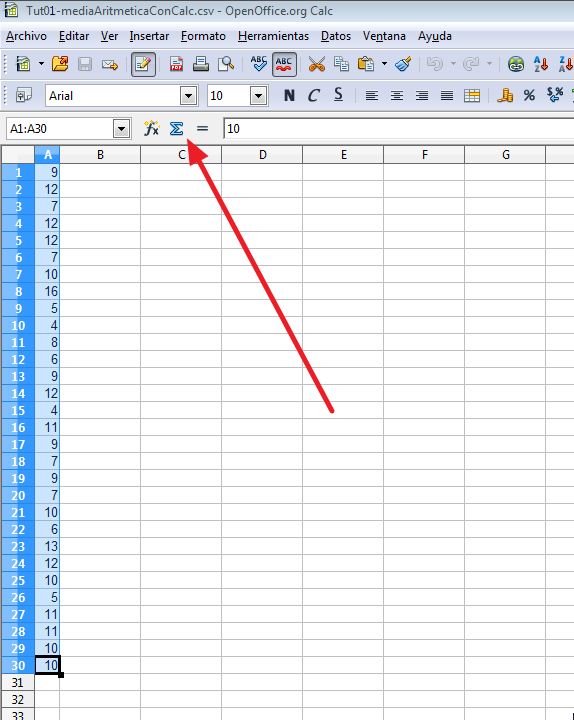
\includegraphics[height=10cm]{../fig/Tut01-Calc-Formula-15.png}
    \end{center}
y después haz clic sobre el símbolo de sumatorio $\Sigma$ de la barra de herramientas, al que señala la flecha roja de la figura. Al hacerlo aparecerá el número 274 en la celda {\tt A31}, inmediatamente debajo del rango que ocupan los números que sumamos. Este es el procedimiento más rápido, pero no es el más flexible. En particular, a veces queremos más libertad a la hora de colocar el resultado de la suma en otras celdas, o sólo queremos sumar una parte del rango, etcétera. Para aprender a controlar más el proceso, fíjate en la fórmula que Calc ha introducido en la celda {\tt A31}, que puedes ver en la línea de entrada.
    \begin{center}
    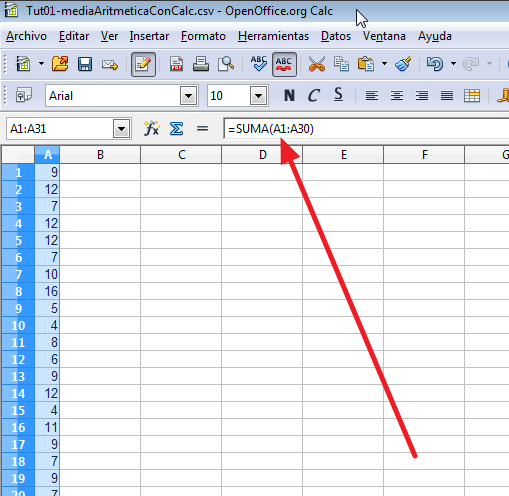
\includegraphics[height=8cm]{../fig/Tut01-Calc-Formula-16a.png}
    \end{center}
Verás que esa fórmula dice {\tt =SUMA(A1:A30)}. A estas alturas, empieza a resultar muy fácil de entender. Calc está usando una función llamada {\tt SUMA}, aplicada a todo el rango, de la misma forma que hicimos con {\tt MIN} o {\tt MAX}. Para ver la diferencia con el método anterior, sitúate en cualquier celda de otra columna (yo voy a usar la {\tt C7}) e introduce allí la misma fórmula:
\begin{center}
{\tt =SUMA(A1:A30)}
\end{center}
El resultado, naturalmente, vuelve a ser 274.
    \begin{center}
    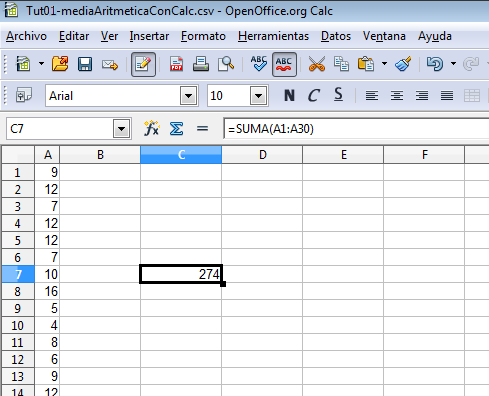
\includegraphics[height=9cm]{../fig/Tut01-Calc-Formula-17.png}
    \end{center}
Ahora, antes de acabar el cálculo de la media, vamos a hacer un pequeño experimento. Asegúrate de que la celda que hayas usado (para mi la {\tt C7}) está seleccionada, y haz clic en la línea de entrada; en ese momento verás que el contenido de la celda se muestra de otra manera.

A continuación, cambia la fórmula de la línea de entrada por esta:
\begin{center}
{\tt =SUMA(A5:A8)}
\end{center}
y pulsa {\tt Entrar}. Debe aparecer 45, y si miras el contenido del rango {\tt A5:A8} verás que, en efecto, es:
\[12 + 7 + 10 + 16 = 45.\]
Como último paso del experimento, selecciona de nuevo la celda que hayas usado, cópiala y pégala (por ejemplo con {\tt CTRL+C, CTRL+V}) en la de debajo (en mi caso, copio la {\tt C7} en {\tt C8}). El resultado es 38.

\begin{ejercicio}
\quad
¿Por qué ha sucedido esto?

\qed
\end{ejercicio}


\vspace{3cm}
\begin{center}
  \textcolor{red}{\Large\bf ¡No sigas, hasta no haberlo intentado entender al menos!}
\end{center}
\newpage


Si no lo ves claro, la flecha roja de la figura te da la pista que necesitas para entender lo que ha pasado:
    \begin{center}
    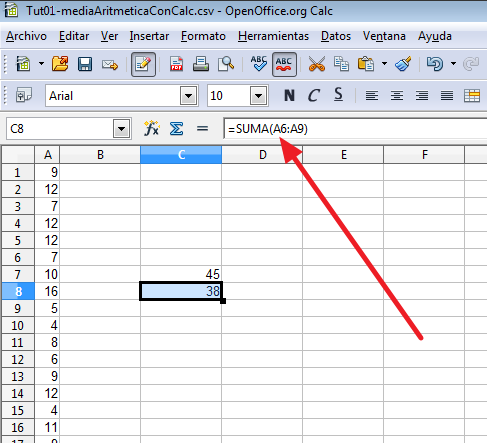
\includegraphics[height=9cm]{../fig/Tut01-Calc-Formula-18.png}
    \end{center}

Volviendo al cálculo de la media, el resultado es, ahora, inmediato. Puedes usar esa cualquier celda, en la que introducimos esta fórmula:
\begin{center}
{\tt =SUMA(A1:A30)/30}
\end{center}
y al pulsar {\tt Entrar} obtendrás $9.133$ como valor de la media (con cuatro cifras significativas, recuerda el Capítulo 1).

Hay otra forma de calcular la media. Siendo una operación esencial en Estadística, Calc no puede sino incluir una función que calcula directamente la media de los valores de cierto rango. Esa función, lamentablemente, no se llama {\tt MEDIA} o algo parecido, sino {\tt PROMEDIO} (en inglés la situación es parecida; en lugar de {\tt MEAN}, se llama {\tt AVERAGE}). Para ver a esta función actuando, selecciona cualquier celda (yo he usado {\tt C10}), y escribe la fórmula:
\begin{center}
{\tt =PROMEDIO(A1:A30)}
\end{center}
El resultado (sorpresa, sorpresa) es $9.133$.

Nos imaginamos que puedes estar preguntándote, ¿y si puedo calcular la media en un sólo paso con {\tt PROMEDIO}, a cuento de qué nos has estado enredando con sumas por aquí, sumas por allá? La respuesta, en el próximo apartado.

Debes guardar esta hoja de cálculo (¡cuidado! ¿qué debes recordar?), porque vamos a trabajar con ella varias veces en esta sesión, y usaremos el resultado que hemos obtenido. Pero te recomiendo que borres el 274 de {\tt A31} para evitar errores más adelante. Basta con que selecciones esa celda y pulses {\tt Supr}. Recuerda grabar los cambios, nosotros hemos llamado al fichero {\tt Tut01-mediaAritmeticaConCalc.ods}. Pero no cierres la hoja de cálculo, porque vamos a seguir usándola a continuación.


\subsection{Media aritmética a partir de una tabla de frecuencias.}
\label{tut02:sec:mediaAritmeticaConTablaFrecuencias}

Vamos a calcular la media aritmética a partir de una tabla de frecuencias, así que empezamos fabricando una.
\begin{ejercicio}
\quad\\
Recuerda lo que aprendimos en la Sección \ref{tut01:sec:TablasFrecuenciaSencillas}, para obtener una tabla de frecuencias de los treinta valores de la hoja {\tt Tut01-mediaAritmeticaConCalc.csv} que estamos usando. ¡Manos a la obra, ya sabes hacerlo!
\qed
\end{ejercicio}

\quad\\
\begin{center}
  \textcolor{red}{\Large\bf ¡No sigas, hasta que tengas esa tabla de frecuencias!}
\end{center}
\newpage

El resultado está en esta figura, en el rango {\tt G3:H15}:
    \begin{center}
    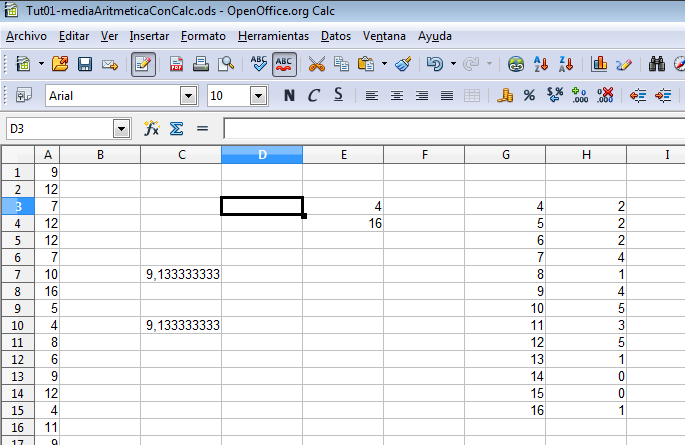
\includegraphics[height=10.5cm]{../fig/Tut01-Calc-Formula-19.png}
    \end{center}
Ahora vamos a imaginar que no tenemos los datos originales, sólo esta tabla de frecuencias, y vamos a calcular la media a partir de esa información. Para aprender un truco nuevo, y hacer más realista el experimento, haz clic con el botón derecho sobre la letra {\tt A} que encabeza esa columna, y luego haz clic en {\tt Ocultar}:
    \begin{center}
    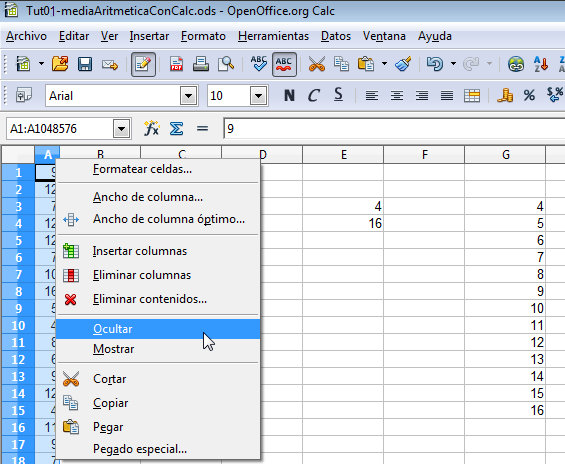
\includegraphics[height=9cm]{../fig/Tut01-Calc-Formula-20.png}
    \end{center}
Al hacerlo verás que la columna {\tt A} parece haber desaparecido. En realidad sigue ahí (y las operaciones que dependen de ella no se ven afectadas), pero no es visible. Puedes hacerla aparecer ahora mismo con {\em deshacer} (recuerda {\tt Ctrl+Z, Ctrl+Y}). O, más adelante, haciendo clic en la esquina superior izquierda (se seleccionará toda la hoja de cálculo), y haciendo después clic con el botón derecho en la columna {\tt B} para seleccionar {\tt mostrar} en el menú contextual que aparece.
    \begin{center}
    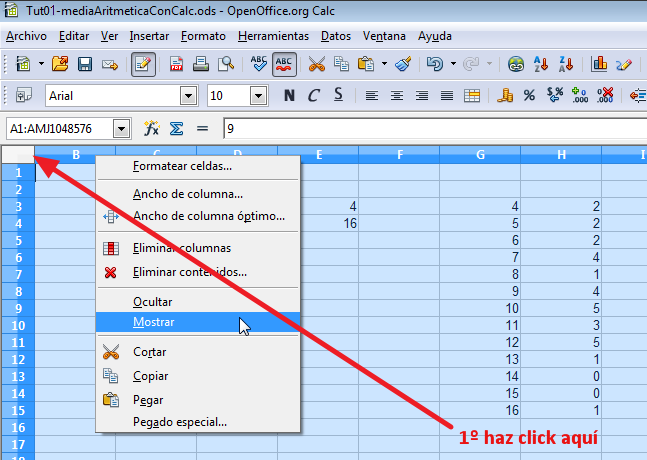
\includegraphics[height=9cm]{../fig/Tut01-Calc-Formula-21.png}
    \end{center}
Volvamos al tema de la media. La fórmula que vamos a usar, en este caso, es esta:
       \begin{center}
        \[
        \bar x=\dfrac{x_1\cdot f_1+x_2\cdot f_2+\cdots+x_k\cdot f_k}{f_1+f_2+\cdots+f_k}=
        \dfrac{\displaystyle\sum_{i=1}^k x_i\cdot f_i}{\displaystyle\sum_{i=1}^k f_i}
        \]
        \end{center}
Es decir, que tenemos que dar estos cuatro pasos:
\begin{enumerate}
  \item Multiplicar cada valor por la correspondiente frecuencia.
  \item Sumar el resultado de todas esas multiplicaciones. Eso dará como resultado el numerador.
  \item Sumar todas las frecuencias. Eso dará como resultado... ¿qué crees que saldrá? Lo haremos, sobre todo, para comprobar que no ha habido errores al hallar las frecuencias. Eso nos dará el denominador.
  \item Dividir para obtener la media.
\end{enumerate}

Pero antes, vamos a practicar la excelente costumbre de añadir comentarios a los datos, para evitar errores, y para que cuando volvamos a verlos (nosotros u otras personas), dentro de dos días, todavía podamos entender lo que nos traíamos entre manos. Insistiremos a lo largo del curso en la idea de que los análisis de datos no documentados son tan buenos como si no existieran. En mi caso, los datos están el columna {\tt G} y sus frecuencias en la {\tt H}, así que añado rótulos descriptivos en la parte superior de la tabla. Basta hacer clic en cada celda y escribir la palabra o frase que queramos (en este caso sin el {\tt =}, porque no es una fórmula).
    \begin{center}
    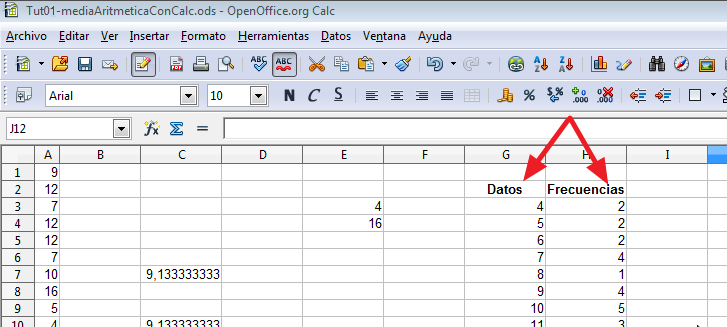
\includegraphics[height=5cm]{../fig/Tut01-Calc-Formula-22.png}
    \end{center}

Ahora vamos con el primero de los cuatro pasos. En la columna {\tt I} (conviene usar esta, para simplificar), hago clic en {\tt I3} y tecleo {\tt =} para comenzar con una fórmula. Después de escribir {\tt =} hago clic con el ratón en {\tt G3} (y veo que el nombre de esa celda aparece en {\tt H3}, a continuación del {\tt =}).
    \begin{center}
    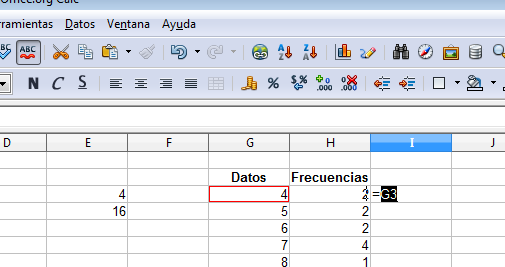
\includegraphics[height=5cm]{../fig/Tut01-Calc-Formula-23.png}
    \end{center}
Sin hacer clic en ningún otro sitio, tecleo un asterisco (que representa la multiplicación), y acto seguido hago clic en {\tt H3}, que aparece en {\tt I3}.
    \begin{center}
    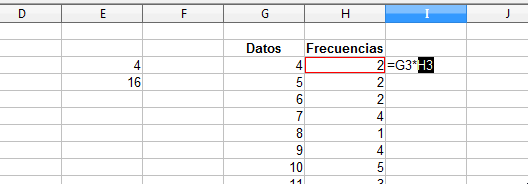
\includegraphics[height=3cm]{../fig/Tut01-Calc-Formula-24.png}
    \end{center}
Lo que hemos hecho, en este caso, es introducir una fórmula seleccionando con el ratón las celdas que intervienen, en lugar de teclear sus nombres. Cuando te acostumbras, resulta una forma bastante cómoda de trabajar. Ya podemos pulsar {\tt Entrar}, y ver el resultado, que es naturalmente 8. Lo que viene a continuación es algo ya conocido. Copiamos y pegamos la fórmula de {\tt I3} en las celdas del rango {\tt I4:I15} (por ejemplo, haciendo clic en el pequeño cuadrado negro de la esquina inferior derecha y arrastrando). El resultado debe ser este:
    \begin{center}
    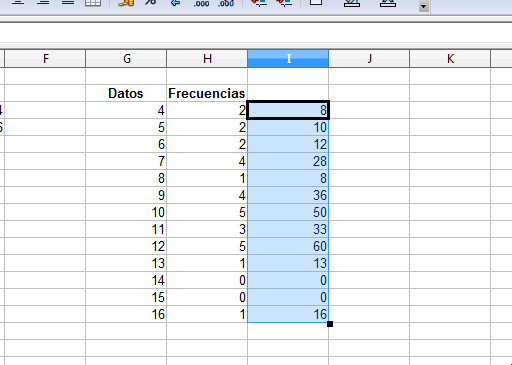
\includegraphics[height=7cm]{../fig/Tut01-Calc-Formula-25.png}
    \end{center}
El segundo paso consiste en sumar los valores que acabamos de obtener. Pero ya hemos aprendido varias formas de sumar los números de una columna. ¿Recuerda el lector que, al final del apartado anterior, le dijimos que ya veríamos la necesidad de aprender a hacer estas sumas? Ahora es el (primer) momento en que las necesitamos. En cualquier caso, el mejor sitio para colocar esa suma
es, probablemente, la celda {\tt I17} debajo, pero no pegado a los datos, para distinguirlo y poder rotularlo. El resultado es 274, que es el numerador de la fórmula de la media. Hemos añadido a la figura varias flechas, para señalar varios aspectos en los que creemos que debes reparar.
    \begin{center}
    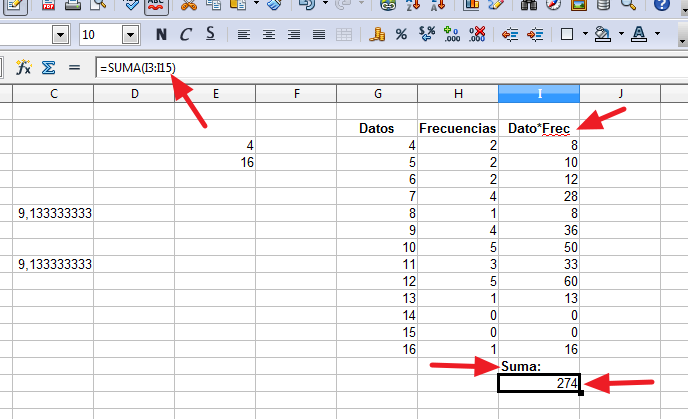
\includegraphics[height=7cm]{../fig/Tut01-Calc-Formula-26.png}
    \end{center}
En el tercer paso sumamos las frecuencias. Después de la discusión previa, no sorprenderá saber que el resultado lo vamos a colocar en {\tt H17}. Hacemos clic en esa celda e introducimos (de la manera que más te guste) la fórmula:
\begin{center}
{\tt =SUMA(H3:H15)}
\end{center}
El resultado (¡como no podía ser de otro modo! ¿por qué?) es 30, el denominador de la fórmula.

Y, finalmente, tenemos que hacer la división para obtener la media. Hacemos clic, por ejemplo, en {\tt I21} e introducimos la fórmula:
\begin{center}
{\tt =I17/H17}
\end{center}
 Al pulsar {\tt Entrar} no hay sorpresa, el resultado es 9,133, como ya obtuvimos en el apartado anterior.
    \begin{center}
    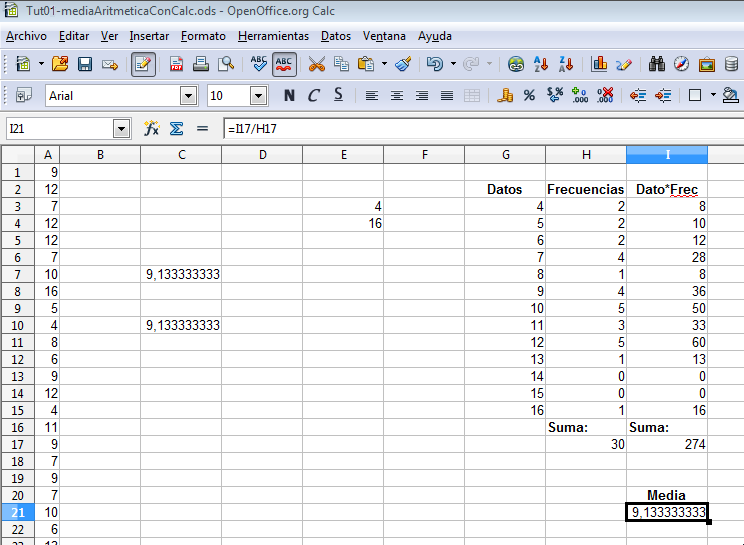
\includegraphics[height=9cm]{../fig/Tut02-27.png}
    \end{center}
Acuérdate de guardar el fichero {\tt Tut01-mediaAritmeticaConCalc.ods} con estos cálculos, lo vamos a necesitar más adelante.


\subsection{El caso de valores agrupados.}
\label{tut02:subsec:mediaAritmeticaDatosAgrupados}

En las {\em Observaciones adicionales} de la  página \pageref{tut01:subsubsec:ObservacionesAdicionalesTablasFrecuenciaSencillas} hemos dejado pendiente la tarea de obtener la tabla de frecuencia de las variable {\tt var2} en la tabla de datos {\tt Tut01-PracticaConCalc.csv}. Ese va a ser el trabajo de la próxima sección. Pero, antes de hacer esto, vamos a pedir al lector que practique lo que ya hemos aprendido sobre el cálculo de la media aritmética.

\begin{ejercicio}
\quad
Carga el archivo {\tt Tut01-PracticaConCalc.ods}, con la tabla de frecuencias que ya hicimos para {\tt var3}
%(ver la Sección \ref{tut01-tut01:subsec:PonASalvoTuTrabajo} del Tutorial01, en la página \pageref{tut01-tut01:subsec:PonASalvoTuTrabajo} de ese tutorial)
, y calcula la media de esa variable por los dos métodos que hemos visto (con y sin tabla de frecuencia). Debes obtener 5.040 (com cuatro cifras significativas). Si quieres guardar el resultado, hazlo con otro nombre, porque volveremos a usar el archivo {\tt Tut01-PracticaConCalc.ods}.
\qed
\end{ejercicio}

Si has hecho el ejercicio que se pedía al final de la anterior sesión, tendrás cargado en Calc el fichero {\tt Tut01-PracticaConCalc.ods}. Y seguramente has ocupado algunas columnas con los cálculos de la media de {\tt var3}. Nosotros vamos a empezar otra vez a partir del fichero {\tt csv} original (que está adjunto en la página \pageref{tut01:sec:TablasFrecuenciaSencillas}), así que, si quieres, haz lo mismo (y luego grabaremos nuestro trabajo de esta sección en formato {\tt ods}, con otro nombre). Nuestro punto de partida, por tanto, es así:
    \begin{center}
    \includegraphics[height=9cm]{../fig/Tut02-28.png}
    \end{center}
Lo primero que tenemos que hacer es calcular el {\sf rango} de {\tt var2}, es decir, el mínimo y máximo de esa variable. Puesto que los valores de {\tt var2} ocupan las celdas {\tt B2:B1301}, es fácil obtener estos valores usando {\tt MIN} y {\tt MAX}:
    \begin{center}
    \includegraphics[height=9cm]{../fig/Tut02-29.png}
    \end{center}
Antes de seguir adelante, nosotros hemos grabado el fichero en formato {\tt ods}, con nombre
    \begin{center}
    {\tt Tut01-mediaAritmeticaVar2.ods},
    \end{center}
para no correr riesgos.\\

Ahora tenemos que dividir el rango en intervalos (clases). ¿Cuántas clases? No vamos a dar, como hemos dicho en la teoría, reglas fijas para esto: ni muchas, ni pocas.  En este caso en particular, vamos a usar diez clases. Concretando, los diez intervalos que vamos a usar son estos (cada desigualdad define un intervalo):
\[x \leq 11,\quad 11 < x \leq 21,\quad 21 < x \leq 31,\quad \ldots \quad 91 < x \leq 101.\]
En este paso es \underline{fundamental} asegurarse de que los intervalos cubren todo el rango de los valores. Por eso hemos llegado a 101.

¿Cómo le explicamos a Calc que queremos usar estos intervalos? Afortunadamente es muy fácil. Basta con colocar en una columna los extremos de los intervalos, así:
    \begin{center}
    \includegraphics[height=7cm]{../fig/Tut02-30.png}
    \end{center}
Los extremos de los intervalos ocupan las celdas del rango {\tt G5:G14}. A continuación, usamos la función {\tt FRECUENCIA}, con la que ya estamos familiarizados, para obtener la tabla de frecuencias en el rango adyacente {\tt H5:H14}. No olvides que antes de usar {\tt FRECUENCIA} tienes que haber seleccionado {\em todas} las celdas del rango {\tt H5:H14}. De lo contrario, se producirán errores. Las dos siguientes figuras resumen el proceso. El cuadro de diálogo de la función es:
    \begin{center}
    \includegraphics[width=15cm]{../fig/Tut02-31.png}
    \end{center}
Y el resultado es:
    \begin{center}
    \includegraphics[width=12cm]{../fig/Tut02-32.png}
    \end{center}
Para entender el resultado lo mejor es un ejemplo: la celda {\tt G8} contiene el valor 40 (y, por supuesto, {\tt G7} contiene 30). Así que Calc coloca en la celda {\tt H8} el número de datos (del total de 1300) que caen en el intervalo:
\[31 < x \leq 41,\]
que, en este ejemplo, resultan ser 131. Y hace lo mismo con todas las demás celdas de la tabla de frecuencia. Sólo la primera, {\tt H5}, es especial, porque en ese caso no hay límite inferior, y puesto que {\tt G5} contiene 10, Calc coloca ahí los valores del intervalo
\[x \leq 11.\]
Ya tenemos la tabla de frecuencias de {\tt var2}. ¡No olvides rotular las columnas de la tabla! El siguiente paso, para calcular la media, es obtener las {\sf marcas de clase} para cada uno de los intervalos. Las vamos a colocar en la siguiente columna, en el rango {\tt I5:I14}. Vamos a empezar con un caso fácil, y dejamos la complicación para el final. En el Capítulo 2 hemos dicho que la marca de clase de un intervalo de la forma $(a,b]$ es el valor:
\[\dfrac{a+b}{2}.\]
Por ejemplo, para nuestro intervalo $(31,41]$, es decir $31 < x \leq 41$, eso significa que la marca de clase es:
\[\dfrac{31+41}{2}=36.\]
Para obtener las marcas de clase en Calc, en todos los casos salvo en el del primer intervalo, usamos la traducción directa de estas operaciones al lenguaje de Calc. Es decir, en {\tt I6} colocamos la fórmula:
\begin{center}
{\tt =(G6+G5)/2}
\end{center}
y copiamos esta fórmula en {\tt I7:I14}. En la figura se muestra el resultado.
    \begin{center}
    \includegraphics[width=12cm]{../fig/Tut02-33.png}
    \end{center}
¿Y para el primer intervalo, que es $x\leq 11$? Bueno, si se observan nuestros datos, veremos que son todos positivos. Así que podríamos asumir que el intervalo es:
\[0 < x \leq 11.\]
Esto no está mal, aunque tiene el inconveniente de que todos los demás intervalos son de longitud 10, y este sería de longitud 11. No hay, en principio, ninguna regla que nos obligue a tomar todos los intervalos de la misma longitud. Pero, puesto que el mínimo de los datos es $1.249$, no hay inconveniente alguno en usar como intervalo:
\[1 < x \leq 11,\]
y obtener como marca de clase $6$.  Para ello introducimos en {\tt I5} la fórmula:
\begin{center}
{\tt =(G5+1)/2}
\end{center}
A partir de aquí el resto de las operaciones son conocidas: multiplicamos las marcas de clase por las frecuencias, sumamos estos productos (la suma es el numerador de la media), después sumamos las frecuencias (para comprobar que en el denominador se obtiene 1300, ¡no se te ocurra saltarte esto y usar directamente 1300!), y finalmente hacemos la división. La figura muestra el resultado de todos estos pasos:
    \begin{center}
    \includegraphics[width=12cm]{../fig/Tut02-34.png}
    \end{center}
Y la media que se obtiene es $51.68$ (con cuatro cifras significativas).

Naturalmente, también podemos calcular la media sin agrupar, directamente a partir de los datos. Podemos sumar toda el rango {\tt B2:B1301} y dividir por 1300, o bien podemos aplicar directamente la función {\tt PROMEDIO} a ese mismo rango.

\begin{ejercicio}
\quad\\
Calcula la media aritmética por esos dos procedimientos.
\qed\\
\end{ejercicio}

\begin{center}
  \textcolor{red}{\LARGE\bf  ¡No sigas, si no has hecho este ejercicio!}
\end{center}

\newpage

El resultado, el mismo en ambos casos, es $51.77$ con cuatro cifras significativas. ¡Y no coincide con el que hemos obtenido a partir de la tabla de frecuencias! Y no es que nos hayamos equivocado, es así. Es el momento de pararse a pensar por qué sucede esto. Y si al cabo de un rato no llega la inspiración, hay que releer el Ejemplo \ref{curso-cap02:ejem:MediaAritmeticaDesdeValoresAgrupadosClases} (pág. \pageref{curso-cap02:ejem:MediaAritmeticaDesdeValoresAgrupadosClases}) del libro.

%\textcolor{red}{\large Hay 131 valores $x$ \\
%con $31<x\leq 41$}

\section{Medidas de posición: mediana, percentiles, moda.}
\label{tut01:sec:MedidasPosicion}

Vamos a continuar nuestro trabajo, aprendiendo lo necesario sobre la forma de obtener, en Calc, las medidas de posición (mediana, cuantiles, percentiles) y las tablas de frecuencia relativas y acumuladas. Aparte de su interés en Estadística, estas operaciones nos van a brindar nuevas oportunidades de practicar las operaciones propias de la hoja de cálculo.

\subsubsection*{La mediana}
\label{tut01:subsubsec:Mediana}

Vamos a volver a trabajar sobre el fichero (adjunto en la página \pageref{tut01:subsec:MediaAritmeticaCalculoDirecto})
\begin{center}
{\tt Tut01-mediaAritmeticaConCalc.csv},
\end{center}
que hemos usado en las dos secciones anteriores. Lo cargamos en Calc, y en la celda {\tt C2} introducimos la fórmula
\begin{center}
{\tt =MEDIANA(A1:A30)}
\end{center}
Obtendrás 9.5 como resultado. Para ver por qué, es necesario ordenar los datos del rango {\tt A1:A30}. Selecciona ese rango con el ratón y usa el menú {\tt Datos} $\to$ {\tt Ordenar}.
    \begin{center}
    \includegraphics[height=9cm]{../fig/Tut03-01.png}
    \end{center}
En el cuadro de diálogo que aparece, asegúrate de que aparece seleccionada la columna {\tt A} y el sentido {\tt ascendente} (de menor a mayor). Pulsa aceptar y obtendrás una lista de valores ordenados en el rango {\tt A1:A30}. Puesto que tenemos $n=30$ valores, debemos mirar a las celdas {\tt A15}, que contiene 9, y {\tt A16}, que contiene 10, para comprender porque la mediana es $9.5$. Dos comentarios sobre la herramienta de ordenación de Calc:
\begin{itemize}
  \item En el futuro puede que quieras ordenar una {\em tabla}, con varias columnas de datos, en la que todos los datos de una fila forman una cierta unidad, y por lo tanto las filas deben conservarse para no perder información. En ese caso, antes de usar {\tt ordenar}, debes asegurarte de que toda la tabla está seleccionada, y después debes elegir cuál de las columnas de la tabla se usa para ordenarla.
  \item Recuerda que puedes deshacer (y rehacer) esta operación si es necesario.
\end{itemize}

\subsubsection*{Cuartiles y percentiles.}
\label{tut01:subsubsec:CuartilesPercentiles}


Ahora, con los datos todavía ordenados, vamos a preguntarnos cuál sería el primer cuartil. La idea informal es que, al igual que la mediana deja por debajo el 50\% de los datos, el primer cuartil debería dejar por debajo el 25\%. Y puesto que $30/4=7.5$, miramos las celdas $\tt A7$ y $\tt A8$. Ambas contienen un 7, así que es de esperar que ese primer cuartil valga 7. Y en efecto, si tecleamos en la celda {\tt C4} la fórmula:
\begin{center}
{\tt =CUARTIL(A1:A30;1)}
\end{center}
obtendremos como respuesta 7. Fíjate en que la fórmula tiene dos argumentos, separados por punto y coma. El primero es el rango del que calculamos el cuartil, y el segundo es el tipo de cuartil que calculamos. Usamos 1 para el primer cuartil, 3 para el tercer cuartil, y 2 para la mediana.
De la misma forma se deduce que el tercer cuartil es 11. Ahora vamos a buscar un percentil, por ejemplo el percentil 66. Con la misma idea informal que antes, este valor deja por debajo el 66\% de los valores. Y puesto que $30\cdot 0.66=19.8$, miramos las celdas {\tt A19} y ${\tt A20}$, que contienen ambas 10. ¿Cuál crees que va a ser el percentil 66? Preguntemos a Calc. Introducimos, en {\tt Calc} la fórmula
\begin{center}
{\tt =PERCENTIL(A1:A30;0,66)}
\end{center}
Ahora nos debemos fijar en que los porcentajes se indican como ``tantos por uno'' (y recuerda que desdichadamente Calc, en español, sigue la costumbre de usar la coma para los decimales). El resultado, como muestra la figura, es $10.14$.
    \begin{center}
    \includegraphics[height=9cm]{../fig/Tut03-03.png}
    \end{center}
¿De dónde sale un número como $10.14$? Nos hemos entretenido en este ejemplo, sobre todo para hacer al lector consciente de esta situación. Queremos advertir, desde el principio, que el cálculo de los cuartiles y percentiles no es tan sencillo como parece sugerir la idea informal con la que hemos empezado el trabajo. Hay muchas formas distintas de definir los percentiles (por ejemplo, el programa R ofrece nueve formas distintas de calcularlos), dependiendo del fin que se les vaya a dar. En la Sección \ref{curso-cap02:subsec:CuartilesPercentiles} (pág. \pageref{curso-cap02:subsec:CuartilesPercentiles}) del libro puedes encontrar más referencias sobre este asunto.\\

Antes de abandonar este apartado, sólo queremos comentar que en Calc existe una función {\tt MODA}, cuyo funcionamiento debería ser evidente.

\subsection{Tablas de frecuencias relativas y acumuladas.}
\label{tut01:subsec:TablasFrecuenciaRelativasAcumuladas}

Para este apartado usaremos el  fichero
\begin{center}
{\tt Tut01-PracticaConCalc.ods},
\end{center}
que obtuvimos en la Sección \ref{tut01:sec:TablasFrecuenciaSencillas}. En ese fichero tiene que estar guardada la tabla de frecuencias de una variable {\tt var3}, que ocupa el rango  {\tt C2:C1301} de la hoja de cálculo. Por eso, al abrir el fichero nos encontraremos en una situación parecida a esta:
    \begin{center}
    \includegraphics[height=8cm]{../fig/Tut03-04.png}
    \end{center}
Vamos a empezar por calcular las frecuencias relativas en el rango {\tt I2:I18}.  Esto es muy fácil, porque cada una de esas frecuencias es igual a la correspondiente frecuencia absoluta, dividida por el número de datos (1300).  Así que introducimos en {\tt I2} la fórmula
\begin{center}
{\tt =H2/1300}
\end{center}
y copiamos esa fórmula en el resto del rango {\tt I2:I18}. No olvides rotular la columna {\tt I}. El resultado será algo como:
    \begin{center}
    \includegraphics[height=8cm]{../fig/Tut03-05.png}
    \end{center}
Antes de seguir vamos a comprobar que las cosas parecen bien hechas. Sitúate en {\tt I20} y calcula la suma de las frecuencias relativas. Si lo hemos hecho bien, esa suma debe ser 1.

Ahora vamos con las frecuencias acumuladas, que son algo más difíciles. Las vamos a situar en el rango {\tt J2:J18}. Vamos a recordar que si $f_1,\ldots,f_k$ son las frecuencias absolutas, y $f''_1,\ldots,f''_k$ son las acumuladas, se cumple esta relación (ver el Capítulo \ref{curso-cap:ValoresCentralesDispersion}, página \pageref{curso-cap02:subsubsec:MedianaTablasFrecuenciasRelativasAcumuladas} del libro):
\[f''_1=f_1,\quad f''_2=f_2+f''_1,\quad f''_3=f_3+f''_2,\ldots,f''_k=f_k+f''_{k-1}.\]
Esta relación es la que vamos a usar en Calc. En la celda {\tt J2} escribimos la fórmula:
\begin{center}
{\tt =H2}
\end{center}
porque en {\tt H2} es donde está $f_1$. Y ahora, en {\tt J3} vamos a usar la relación:
\[f''_2=f_2+f''_1\]
para obtener $f''_2$. Ya sabemos que $f_2$ está en {\tt H3}. ¿Dónde está $f''_1$? Lo acabamos de poner en {\tt J2}. Así que la fórmula es:
\begin{center}
{\tt =H3+J2}
\end{center}
Lo bueno de proceder así es que ahora esa fórmula se puede copiar desde {\tt J3} a las restantes celdas del rango (es decir, a {\tt J4:J18}) y se obtienen todas las frecuencias acumuladas. El resultado es:
    \begin{center}
    \includegraphics[height=8cm]{../fig/Tut03-06.png}
    \end{center}
y, naturalmente, la última de las frecuencias acumuladas es igual a $n=1300$.

Ya sólo nos quedan las frecuencias relativas acumuladas. Dejamos este último paso como ejercicio para el lector. El resultado debe ser el de la figura:
    \begin{center}
    \includegraphics[height=8cm]{../fig/Tut03-07.png}
    \end{center}

\begin{ejercicio}
\quad\\
\begin{enumerate}
  \item Obtén esa tabla de frecuencias relativas acumuladas.
  \item Usando esa tabla de frecuencias relativas acumuladas, calcula la mediana de {\tt var3}.
  \item Confirma la respuesta usando la función {\tt MEDIANA} de Calc.
\end{enumerate}
\qed
\end{ejercicio}


Cuando los datos se presentan agrupados por intervalos, los cálculos son similares, pero utilizando las marcas de clase. No entraremos en detalles.

\section{Varianza y desviación típica.}
\label{tut01:sec:Varianza}

Hemos recorrido ya una buena parte de nuestra introducción a la Estadística Descriptiva con la hoja de cálculo Calc. Para concluir este tutorial, vamos a aprender a calcular la varianza y desviación típica (poblacionales) con Calc. También aprenderemos a calcular la cuasivarianza y la cuasidesviación típica  (muestrales). No te preocupes si todavía no entiendes por qué es necesaria esta diferencia entre poblacional y muestral, ya se aclarará más adelante. De momento, lo único importante es que sepas que hay dos tipos de objetos, y que te fijes en cuál estamos calculando en cada caso. Al principio del curso el protagonismo es para las cantidades poblacionales, pero poco a poco los muestrales irán ganando en importancia.\\

Sea $x=(x_1,\ldots,x_n)$ un vector de datos (no agrupados). La fórmula de la varianza poblacional es:
\[
Var(x)=\dfrac{\displaystyle\sum_{i=1}^n(x_i-\bar x)^2}{n}.
\]
El valor $\bar x$ representa la media de $x$, así que este cálculo {\em presupone} que ya hemos calculado la media de $x$. Como en casos anteriores, podemos ver esta fórmula como una receta para realizar, en varios pasos, el cálculo correspondiente:
\begin{enumerate}
  \item Como hemos dicho, debemos haber calculado la media $\bar x$.
  \item Debemos restarle la media $\bar x$ a cada uno de los valores $x_i$.
    \[(x_1-\bar x), (x_2-\bar x),\ldots, (x_n-\bar x).\]
  \item Después elevamos cada diferencia al cuadrado, para obtener los $n$ valores
  \[(x_1-\bar x)^2, (x_2-\bar x)^2,\ldots, (x_n-\bar x)^2.\]
  \item Sumamos los cuadrados y
  \item Dividimos por $n$.
\end{enumerate}
Como se ve, buena parte del trabajo consiste en aplicar la misma operación a toda una lista de valores, y eso hace que esta tarea sea fácil de abordar con una hoja de cálculo como Calc. Y, al igual que sucedía con la media, el cálculo se puede hacer de varias formas distintas, dependiendo del punto de partida y de nuestros deseos.\\

Para practicar con un ejemplo vamos a volver al mismo punto del comienzo de la Sección \ref{tut01:subsec:MediaAritmeticaCalculoDirecto} (página \pageref{tut01:subsec:MediaAritmeticaCalculoDirecto}), es decir, que volvemos a cargar el fichero
\begin{center}
{\tt Tut01-mediaAritmeticaConCalc.csv},
\end{center}
que aparece adjunto en esa página. Cuidado: usamos el {\tt csv}, no el fichero de tipo {\tt ods} que obtuvimos al final de esa sección, y que vamos a usar en breve.


Una vez abierto el fichero, para el primer paso del método vamos a calcular la media otra vez, usando {\tt PROMEDIO} para abreviar.
\begin{ejercicio}
\quad\\
Abre el fichero {\tt csv} y haz ese cálculo de la media. Coloca el resultado, con un rótulo, en las celdas {\tt A31:A32}.
\qed
\end{ejercicio}
\quad\\
\begin{center}
  \textcolor{red}{\LARGE\bf  ¡No sigas, si no has hecho este ejercicio!}
\end{center}

\newpage

El resultado se muestra en la siguiente figura:
    \begin{center}
    \includegraphics[width=10cm]{../fig/Tut02-45.png}
    \end{center}
Obtendrás, como ya sabíamos, $\bar x=9.133$.  Guardamos el fichero en formato {\tt ods}, con nombre, por ejemplo
\begin{center}
{\tt Tut01-varianzaConCalc.ods}\label{tut01:fichero:Tut01-varianzaConCalc.ods}.
\end{center}
Antes de seguir adelante, vamos a insistir en la necesidad de rotular y comentar bien nuestro trabajo. El problema es que, puesto que los datos empiezan en la celda {\tt A1} parece que nos hemos quedado sin sitio para incluir un rótulo. No hay problema, hagamos algo de sitio. Haz clic con el botón derecho del ratón en el número 1 al principio de la primera fila de la hoja de cálculo. En el menú que aparece haz clic en {\tt Insertar filas}, y verás como aparece una fila vacía, y todo el contenido de la hoja se desplaza una posición hacia abajo.
    \begin{center}
    \includegraphics[width=7cm]{../fig/Tut02-46.png}
    \end{center}
Y si necesitas insertar, por ejemplo, cinco filas vacías, empieza seleccionando cinco filas (si lo haces bien, verás sombreada completamentes toda esas filas), antes de usar {\tt Insertar filas}. Se insertarán tantas filas como filas tengas seleccionados. No te preocupes, cuando se inserta una fila, Calc actualiza todas las fórmulas automáticamente, así que, por ejemplo, el cálculo que hemos hecho de la media no se ve afectado. En concreto, puedes comprobar que ahora la media aparece en la celda {\tt A33}, y se calcula con {=PROMEDIO(A2:A31), usando el nuevo rango que ocupan los datos}. Escribamos en la celda {\tt A1} el rótulo {{\tt datos}}.

\subsubsection*{Referencias absolutas en la hoja de cálculo}
\label{tut01:ReferenciasAbsolutasHojaCalculo}

Ahora vamos con el segundo paso, para calcular las diferencias $(x_i-\bar x)$. Vamos a colocarlas en el rango {\tt B2:B31}. Para calcular la primera, nos situamos en la celda {\tt B2}, e introducimos la fórmula:
\begin{center}
{\tt =A2-A33}
\end{center}
Recuerda que la media $\bar x$ está en {\tt A33}. El resultado es $x_1-\bar x=-0.1333$ (con cuatro cifras significativas):
    \begin{center}
    \includegraphics[width=8cm]{../fig/Tut02-47.png}
    \end{center}
Ahora, como hemos hecho en casos anteriores, vamos a copiar esa fórmula a las restantes celdas del rango {\tt B3:B31}. Recuerda que puedes pinchar en el pequeño cuadrado negro de la esquina inferior derecha de {\tt B2} y arrastrar para cubrir todo el rango. Se obtiene (sólo se muestran las primeras filas):
    \begin{center}
    \includegraphics[width=8cm]{../fig/Tut02-48.png}
    \end{center}
Una pequeña luz de alarma se debería encender en algún rincón de nuestra cabeza: si estamos restando $9.133$, ¿cómo es que los resultados son números enteros, sin decimales? Ahora que algo ha llamado nuestra atención, fíjate mejor: los resultados son los datos de partida, sin modificación alguna. ¡Y la razón por la que esto sucede es que estamos restando 0!

Enseguida vamos a ver lo que ha pasado, y a ponerle remedio. Pero queremos llamar la atención del lector sobre el hecho de que es necesario, imprescindible de hecho, preguntarse constantemente por las operaciones que hacemos, si son correctas, incluso tratando de anticipar el resultado para detectar posibles errores o problemas.\\

Veamos cuál ha sido el problema. Hagamos una pequeña comprobación. En la celda {\tt B3} esperamos tener el resultado de {\tt A3}, menos la media $9.133$, que está en {\tt A33}. Es decir, que la fórmula para calcular {\tt B3} tiene que ser:
\begin{center}
{\tt =A3-A33}
\end{center}
Pero si te sitúas en {\tt B3}, verás que la fórmula que aparece en esa celda es:
\begin{center}
{\tt =A3-A34}
\end{center}
De la misma forma, en {\tt B4} tenemos
\begin{center}
{\tt =A4-A35}
\end{center}
Ahora ya debería empezar a estar claro lo que ha pasado: hemos sido víctimas de la forma de actualizar las {\em referencias relativas} en una hoja de cálculo. Cuando copiamos la fórmula de {\tt B2} en {\em la celda de abajo}, todas las referencias a celdas que aparecen en la fórmula se sustituyen por referencias a las correspondientes {\em celdas de abajo}. Y la celda situada debajo de {\tt A33} es {\tt A34}, que contiene nada, es decir un 0. Por eso hemos restado ceros.

De acuerdo, ese es el problema. ¿Y la solución? Calc normalmente utiliza {\em referencias relativas}, pero en ocasiones como esta necesitamos una forma de emplear {\em referencias absolutas}, que apunten a posiciones inmutables dentro de la hoja de cálculo. Afortunadamente, es muy sencillo hacer esto. Empecemos por deshacer los últimos pasos (usando el icono \includegraphics[width=0.5cm]{../fig/Tut02-49.png} de la barra de herramientas de Calc, o con {\tt Ctrl+Z}), hasta dejar la columna {\tt B} libre. Y ahora, en {\tt B2} introducimos la fórmula:
\begin{center}
{\tt =A2-\$A\$33}
\end{center}
con dos símbolos {\tt\$} adicionales. Con cada uno esos símbolos le estamos diciendo a Calc que deje fijo el elemento correspondiente. Es decir {\tt\$A} significa ``no cambies la columna {\tt A}'', y ``\$33'' significa ``no cambies la fila {\tt 33}''. Al introducir esa fórmula, el resultado en {\tt B3} es el mismo que antes (claro), pero cuando copiamos esa fórmula en el resto del rango {\tt B3:B31}, las cosas cambian (a mejor):
    \begin{center}
    \includegraphics[width=8cm]{../fig/Tut02-50.png}
    \end{center}
Antes de avanzar, escribe en {\tt B1} un rótulo para esa columna, por ejemplo, {\tt datos - media}.

De acuerdo, ya hemos superado este escollo, tenemos calculadas las diferencias $x_i- \bar x$ y podemos seguir con el tercer paso, elevando esas diferencias al cuadrado. ¿Cómo se hace esto en Calc? En la mayoría de los lenguajes informáticos, Calc incluido, la operación ``elevar al cuadrado'' se representa mediante la notación {\verb#^2#} (en algunos casos se utiliza {\tt **2}). Así que en la celda {\tt C2} escribimos la fórmula:
\begin{center}
{\verb#=B2^2#}
\end{center}
y la copiamos en el rango {\tt C3:C31}. No te olvides de rotular la columna C.
    \begin{center}
    \includegraphics[width=8cm]{../fig/Tut02-51.png}
    \end{center}
Los últimos pasos son sencillos. Nos situamos en {\tt C33} (serviría cualquier celda libre, pero esta es conveniente) e introducimos la fórmula para sumar todos los valores del rango {\tt C2:C31}. Es decir:
\begin{center}
{\tt =SUMA(C2:C31)}
\end{center}
    \begin{center}
    \includegraphics[width=8cm]{../fig/Tut02-52.png}
    \end{center}
El resultado, $243.5$ (con cuatro cifras significativas) es el numerador de la varianza:
\[\displaystyle\sum_{i=1}^n(x_i-\bar x)^2.\]
Para calcular la varianza sólo tenemos que dividir por 30, cosa que hacemos en la celda {\tt C35}:
    \begin{center}
    \includegraphics[width=8cm]{../fig/Tut02-53.png}
    \end{center}
La varianza, por tanto, es 8.156 (con cuatro cifras significativas).

\subsubsection*{La varianza usando funciones propias de Calc}
\label{tut01:subsubsec:VarianzaConFuncionesPropiasCalc}

Hay otra forma de obtener ese resultado. Puesto que la varianza de un conjunto de datos es un valor que se calcula con mucha frecuencia, Calc incluye una función para obtenerla directamente. Nos situamos en {\tt C37} y usamos el menú {\tt Insertar} $\to$ {\tt Función}. En el cuadro de diálogo que aparece, en {\tt Categoría} elegimos {\tt Estadística} y entonces, en el cuadro {\tt Función} navegamos hacia abajo, hasta el final de la lista de funciones, donde veremos varias funciones cuyo nombre empieza por {\tt VAR}, como en esta figura (los nombres en inglés son los mismos):
    \begin{center}
    \includegraphics[width=7cm]{../fig/Tut02-54.png}
    \end{center}
La que nos interesa ahora es {\tt VARP} (recuerda {\tt VAR}ianza {\tt P}oblacional). La que se llama {\tt VAR} es la cuasivarianza muestral (con $n-1$ en lugar de $n$ en el denominador), que usaremos mucho más adelante en el curso. Las dos versiones con una a al final, las que se llaman {\tt VARA} y {\tt VARPA}, son variantes de estas, que sirven para los casos en los que el conjunto de datos contiene alguna omisión. Este problema de los {\em datos ausentes} ({\em missing data}, en inglés) es uno de los problemas prácticos más frecuentes en Estadística, y a veces influye enormemente en la manera adecuada de proceder. De momento, no obstante, sólo necesitamos {\tt VARP}. La seleccionamos haciendo doble clic sobre su nombre, y en el siguiente paso la aplicamos al rango {\tt A2:A31} así:
    \begin{center}
    \includegraphics[width=7cm]{../fig/Tut02-55.png}
    \end{center}
Obtenemos, en {\tt C37}, el mismo resultado que ya teníamos en {\tt C35}. Y el lector se volverá a preguntar, ¿y no podríamos habernos ahorrado todos estos pasos, entonces? La respuesta es que, en este caso, sí, podríamos haber usado directamente {\tt VARP}. Pero cuando lo que tenemos, como punto de partida, no son los datos, sino una tabla de frecuencias, entonces es necesario seguir pasos parecidos a estos. Ese es, de hecho, casi todo el trabajo que nos falta por hacer en esta sección.\\

\subsubsection*{Desviación y cuasidesviación típica.}
\label{tut01:subsubsec:DesviacionCuasidesviacion}

Pero, antes de ir a eso, un último paso. La {\em desviación típica} (poblacional) es la raíz cuadrada de la varianza (poblacional). La podemos obtener, por tanto, calculando la raíz cuadrada de {\tt C35} (o de {\tt C37}). ¿Cómo se calcula una raíz cuadrada en Calc? Usando la función {\tt RAIZ} (en inglés es {\tt SQRT}, de {\em square root}) Dejamos como ejercicio para el lector comprobar por este método que la desviación típica es 2.849. Hay otra forma, usando la función {\tt DESVESTP}, de desviación estándar poblacional. Hay cuatro funciones que empiezan por {\tt DESVEST}, que son las raíces de las correspondientes {\tt VAR} (sus análogas en inglés tienen nombres que empiezan por {\tt STDEV}, de standard deviation). El siguiente ejercicio para el lector es comprobar que {\tt DESVESTP} produce el mismo resultado que {\tt RAIZ} aplicado a {\tt VARP}.

Acuérdate de guardar tu trabajo de esta sección en un fichero, con formato {\tt ods}, claro. Nosotros lo hemos llamado {\tt Tut01-varianzaConCalc.ods}.

\subsection{Varianza a partir de la tabla de frecuencias.}
\label{tut02:sec:VarianzaTablaFrecuencias}

Volvamos a cargar el fichero {\tt Tut01-mediaAritmeticaConCalc.ods}, que guardaste al final de la Sección \ref{tut02:sec:mediaAritmeticaConTablaFrecuencias}, y que contiene una tabla de frecuencias para los 30 datos con los que hemos trabajado en aquella sección. Vamos a usar ahora esa tabla de frecuencias para calcular la varianza poblacional de los datos (que ya hemos calculado, y sabemos que vale aprox. $8.156$). Cuando los datos se presentan así, en forma de una tabla de frecuencias, no existe una función de Calc, como {\tt VARP}, que nos permita obtener la varianza a partir de la tabla. Así que lo que haremos en estos casos es usar la fórmula:
\[
\dfrac{\displaystyle\sum_{i=1}^k f_i\cdot(x_i-\bar x)^2}{\displaystyle\sum_{i=1}^k f_i}=
\dfrac{f_1\cdot(x_1-\bar x)^2+\cdots+f_n\cdot(x_n-\bar x)^2}{f_1+f_2+\cdots+f_n}
.\]
La siguiente figura resume el trabajo que hay que hacer para conseguir el resultado. Dejamos al lector la tarea de reproducir estos valores. No hay nada nuevo aquí, sólo hay que poner juntas las piezas.
    \begin{center}
    \includegraphics[width=15.5cm]{../fig/Tut02-56.png}
    \end{center}
Hemos destacado en color rojo las novedades con respecto al cálculo de la media, que puedes usar como referencia para completar el primer apartado del siguiente ejercicio:

\begin{ejercicio}
\quad\\
\begin{enumerate}
    \item Repite las operaciones de la anterior figura, hasta completar el cálculo de la varianza.
    \item Calcula la varianza y desviación típica de la variable {\tt var3} del fichero
        \begin{center}
        {\tt Tut01-PracticaConCalc.csv},
        \end{center}
        (adjunto en la página \pageref{tut01:sec:TablasFrecuenciaSencillas}), aplicando la función {\tt VARP} (y {\tt DESVESTP}) directamente sobre los datos.
  \item Vuelve a calcular esos mismos valores a partir de la tabla de frecuencias que obtuvimos en la Sección \ref{tut01:sec:TablasFrecuenciaSencillas}, y que debes tener guardada en el fichero
      \begin{center}
        {\tt Tut01-PracticaConCalc.ods}
      \end{center}
      Compara los resultados con los del apartado anterior.
\end{enumerate}
\qed
\end{ejercicio}

\section{Ejercicios adicionales y soluciones.}
\label{tut01:sec:SolucionesEjerciciosAdicionales}

\subsection*{Ejercicios adicionales.}


\begin{enumerate}
  \addtocounter{enumi}{10}
  \item Queremos saber la edad media de los empleados de una empresa que tiene tres fábricas. La primera fábrica tiene $150$ trabajadores, con una edad media de $32$ años. La segunda tiene $241$ trabajadores con una edad media de $39$ años, y la tercera tiene $165$ trabajadores, con una edad media de $37$ años.  ¿Cuál es la edad media del conjunto de trabajadores de la empresa? Una indicación. La media no es ``la media de las medias'':
      \[\dfrac{32 + 39 + 37}{3}.\]
      Para calcular correctamente la media necesitas algo más parecido a lo que hacemos cuando nos dan una tabla de frecuencias.
  \item Este ejercicio explora una idea similar a la del anterior.
  \begin{enumerate}
    \item   Las calificaciones finales de un estudiante en cuatro asignaturas fueron $82$, $86$, $90$ y $70$. Si los respectivos créditos\footnote{El {\em crédito} es una unidad de medida académica que, en esencia, mide el tiempo de formación del estudiante. Ver \link{http://es.wikipedia.org/wiki/Cr\%C3\%A9dito\_acad\%C3\%A9mico}{http://es.wikipedia.org/wiki/Crédito\_académico}} otorgados a esos cursos son $3$,$5$,$3$ y $1$ determinar una calificación media apropiada. De nuevo, es posible que pienses que la calificación media es:
      \[\dfrac{82 + 86 + 90 + 70}{4},\]
      pero si te preguntamos por la {\em calificación media por crédito}, ¿crees que ese es el resultado correcto? ¿Qué tipo de media es la que estamos calculando aquí?

    \item Supongamos que he hecho un viaje a pie en tres etapas. En la primera etapa he recorrido $25$ kilómetros en $6$ horas. En la segunda he recorrido $21$ kilómetros en $4$ horas y en la tercera, $32$ kilómetros en $7$ horas. ¿Cuál ha sido mi velocidad media en ese viaje, medida en kilómetros por hora? ¿Ves la relación con el apartado anterior?

    \item El átomo de Cloro tiene dos isótopos, cuya masa es de $35$u (unidades de masa atómica) y $37$u, respectivamente. El $75.5\%$ de los átomos de Cloro son isótopos del primer tipo, y el resto son isótopos del segundo tipo. ¿Cuál es la masa atómica media del Cloro?
  \end{enumerate}
  Las medias que aparecen en este ejercicio son ejemplos de {\sf medias ponderadas}, ver el enlace:
  \begin{center}
  \link{http://es.wikipedia.org/wiki/Media_ponderada}{http://es.wikipedia.org/wiki/Media\_ponderada}.
  \end{center}

  \item En la página \pageref{tut01:subsubsec:NumerosAleatoriosCalc} hemos hablado de números pseudoaleatorios con Calc, y hemos presentado la función {\tt ALEATORIO.ENTRE()}. Esta función genera números aleatorios enteros. Si queremos generar números reales no enteros (como los valores de una variable cuantitativa continua) podemos usar la función {\tt ALEATORIO()}. El resultado de esta función es un número pseudoaleatorio entre $0$ y $1$. Vamos a hacer algunos experimentos con ella.
      \begin{enumerate}
        \item Usa la función {\tt ALEATORIO()} para generar 100 números aleatorios entre $0$ y $1$. Calcula su media. Calcula su desviación típica. Repite el proceso varias veces (recuerda {\tt Ctrl + Mays + F9}) y observa los valores de la media y la desviación típica cada vez. ¿Qué observas?
        \item Ahora calcula $100$ números aleatorios entre $30$ y $50$, y repite los pasos anteriores, para observar la media y la desviación típica. Indicación: para generar estos números sólo necesitas multiplicar por $20$ y sumar $30$.
        \item Más ambicioso: trata de construir una hoja Calc en la que, tras introducir dos números $a$ y $b$ (con $a < b$), Calc construya $100$ números pseudoaleatorios del intervalo $(a,b)$ y calcule su media y desviación típica.
      \end{enumerate}

  \item Para percibir algunas de las dificultades que nos vamos a encontrar em el trabajo con los datos, nada como la práctica. El fichero:
      \begin{center}
        \fichero{../datos/Tut01-DatosTemperaturaINE.csv}{Tut01-DatosTemperaturaINE.csv}
      \end{center}
      contiene datos sobre temperaturas medias mensuales registradas en distintos observatorios meteorológicos españoles, desde enero de 2007 a diciembre de 2012. Los datos proceden del INE (Instituto Nacional de Estadística de España, ver \link{http://www.ine.es}{http://www.ine.es}). El fichero, además de la tabla de datos propiamente dicha, contiene varias filas iniciales y varias finales con información adicional sobre los datos. En cuanto a la tabla, daremos algunas indicaciones:
      \begin{itemize}
        \item La primera columna contiene el nombre del observatorio.
        \item La primera fila (la cabecera) contiene el código del mes correspondiente a la observación. Por ejemplo {\tt 2011M09} significa {\em Septiembre de 2011}.
        \item Las columnas se han separado con tabuladores. Los valores aparecen entrecomillados.
        \item Un valor como \verb#"."# significa que ese dato no está disponible, es un dato ausente. EL problema de los datos ausentes (en inglés, {\em missing data}) va a ser uno de nuestros compañeros inseparables en el Análisis de Datos.
      \end{itemize}
      Sabiendo esto:
      \begin{enumerate}
        \item Lee el fichero con Calc. Es muy posible que antes tengas que {\em esquilarlo} un poco.
        \item Calcula la media de las temperaturas en Guadalajara durante ese periodo de tiempo.
        \item Calcula la temperatura media durante el mes de Agosto en todos los observatorios.
      \end{enumerate}


  %% IDEAS:
  % \item %Un fichero csv que sea ``entretenido'', para que lo abran con Calc.
  % \item %Algo sobre media ponderada.

\end{enumerate}


%\subsection*{Soluciones de algunos ejercicios.}


%\paragraph{\bf $\bullet$ Ejercicio \ref{tut02:ejercicio02}, pág. \pageref{tut02:ejercicio02}}
%\label{tut02:ejercicio02:sol}\quad\\
%Al final las variables valen $a=15$, $b=100$, $c=1500$.




\vspace{2cm} \hrule
\quad\\
Fin del Tutorial01. ¡Gracias por la atención!

\newpage
%\includegraphics[width=15cm]{01-02-GuiaDeTrabajo.pdf}
%\includepdf[pages={1-},scale=0.90]{01-02-GuiaDeTrabajo.pdf}



\end{document}
